\documentclass[twoside]{article}
\usepackage{configuracoes}

% ============================================================================
% main.tex
% ============================================================================
% Objetivo:
% Arquivo principal da lista de exercícios.
% Aqui ficam os metadados da lista, escolhas locais de compilação e a ordem
% dos arquivos de exercícios incluídos no documento.
%
% Diretriz de uso:
% - o núcleo do template fica em configuracoes.sty;
% - este arquivo deve concentrar apenas os dados e decisões da lista atual;
% - os enunciados e resoluções devem ficar em arquivos separados (ex1.tex,
%   ex2.tex, ...), para facilitar manutenção e reaproveitamento.
% ============================================================================

% ----------------------------------------------------------------------------
% Idioma principal do documento
% ----------------------------------------------------------------------------
% O pacote babel já foi carregado no .sty com português e inglês disponíveis.
% Como esta lista está escrita em inglês, explicitamos a língua principal aqui.
% Em listas futuras, altere para \selectlanguage{portuguese} se necessário.
\selectlanguage{english}

% ----------------------------------------------------------------------------
% Metadados da lista atual
% ----------------------------------------------------------------------------
% Ponto de personalização do usuário:
% redefina abaixo apenas os dados desta lista. Assim, o template permanece
% reutilizável sem exigir edição do arquivo configuracoes.sty.
\renewcommand{\CodigoDisciplina}{PGF5473}
\renewcommand{\NomeDisciplina}{Introduction to Nonlinear Optics}
\renewcommand{\NumeroLista}{2}

\renewcommand{\titulo}{\NomeDisciplina\ - Exercise Sheet \NumeroLista}
\renewcommand{\professorLista}{Prof.\ Dr.\ Rafael Ferreira Pinto do Rego Barros}
\renewcommand{\autorLista}{Guterman Rodrigues de Araujo Junior -- N\textsuperscript{o} USP 7990464}
\renewcommand{\tituloPDF}{[2026s1] Introduction to Nonlinear Optics - Exercise Sheet 1}
\renewcommand{\autorListaPDF}{Guterman Rodrigues de Araujo Junior -- No USP 7990464}
\renewcommand{\assuntoPDF}{Nonlinear Optics - Exercise Sheet 1}
\renewcommand{\instituicaoLista}{Instituto de F\'isica, Universidade de S\~ao Paulo - SP}
\renewcommand{\dataLista}{20th June 2026}

% Obs: Caso seu template use os comandos \newcommand definidos anteriormente:
\newcommand{\tituloLista}{Exercise Sheet \NumeroLista}
\newcommand{\disciplina}{\CodigoDisciplina\ - \NomeDisciplina}
\newcommand{\professor}{\professorLista}
\newcommand{\dataEntrega}{\dataLista}
\newcommand{\instituicao}{\instituicaoLista}

% ----------------------------------------------------------------------------
% Controles locais de exibição
% ----------------------------------------------------------------------------
% O ambiente resolucao pode ser mostrado ou ocultado sem editar os arquivos dos
% exercícios. Isso permite gerar, a partir da mesma base, uma versão com
% soluções e outra apenas com os enunciados.
\MostrarResolucoes
% \OcultarResolucoes

% ----------------------------------------------------------------------------
% Layout local do documento
% ----------------------------------------------------------------------------
% Observação importante:
% o uso de \begin{multicols*}{1} gerava warning e, na prática, fazia o pacote
% forçar duas colunas. Como a intenção desta lista é uma coluna, o ambiente foi
% removido. Se no futuro você quiser duas colunas de fato, use multicols com 2
% de maneira explícita e consciente.





\usepackage[
  backend=biber,
  style=authoryear,
  sorting=nyt
]{biblatex}

\addbibresource{referencias.bib}

\DeclareCiteCommand{\authorlinkcite}
  {}
  {\printtext[bibhyperref]{\printnames{labelname}}}
  {\multicitedelim}
  {}




\begin{document}
    
    \maketitle
    \thispagestyle{fancy}
    
    % \tableofcontents
    % Ative apenas se fizer sentido para listas longas. Em listas curtas, o custo
    % visual normalmente não compensa.
    
    % ----------------------------------------------------------------------------
    % Exercícios da lista
    % ----------------------------------------------------------------------------
    % Regra prática:
    % - cada arquivo de exercício deve conter apenas conteúdo;
    % - a ordem da lista é definida aqui;
    % - para adicionar novos exercícios, basta criar novos arquivos e incluí-los.
    
    \newif\ifusarDuasColunas
    % \usarDuasColunasfalse
    \usarDuasColunastrue
    
    \ifusarDuasColunas
        \begin{multicols*}{2}
    \fi
        
        % \twocolumn
        % ============================================================================
% ex1.tex
% ============================================================================
% Exercício individual da lista.
% Este arquivo deve conter apenas o conteúdo do exercício e, quando desejado,
% sua resolução. Não deve carregar pacotes nem redefinir configurações globais.
%
% Interface adotada neste exemplo:
% - ambiente `exercicio` com identificador textual livre;
% - ambiente `resolucao` para a solução;
% - subseções internas apenas para organizar a exposição.
% ============================================================================

\begin{exercicio}[Problem 1 --- SHG with Gaussian Beams]
Consider the problem of Second Harmonic Generation (SHG) with Gaussian beams. We have discussed how in this case the effective nonlinear coefficient carries an overlap integral that depends on the matching between the interacting fields.

\begin{enumerate}[a)]
\item Show with a numerical simulation that the Boyd-Kleinman criterion arises from optimizing this overlap integral.
\item Discuss how the phase mismatch is affected when Gaussian beams are used instead of plane waves.
\end{enumerate}
\end{exercicio}

\begin{resolucao}[Solution]

\subsection*{(a) Numerical Optimization of the Overlap Integral}

    \paragraph*{Theoretical Framework}
        The analytical treatment of nonlinear interactions with focused Gaussian beams is given in \textbf{Section 2.10 of \authorlinkcite{Boyd}} (4th edition, \textit{Nonlinear Optical Interactions with Focused Gaussian Beams}, pp.~109--116). In particular, the derivation used here is based on \textbf{Section 2.10.3} (\textit{Harmonic Generation Using Focused Gaussian Beams}, pp.~112--116), where Boyd writes the driven paraxial equation for the generated harmonic field in Eq.~(2.10.7), represents the fundamental Gaussian beam in Eq.~(2.10.8), introduces the harmonic-field trial solution in Eq.~(2.10.9), and obtains the longitudinal generation integral in Eq.~(2.10.11b). The optimum focusing result quoted by Boyd and Kleinman is stated explicitly after Fig.~2.10.4 and summarized in Eq.~(2.10.14), where Boyd reports the optimum values $L/b=2.84$, $\Delta k=3.2/L$, and the numerical coefficient $K=1.068$ for the original Gaussian-units normalization.
    
        The propagation properties of a Gaussian beam are taken from \textbf{Section 3.1 of \authorlinkcite{Saleh}} (\textit{The Gaussian Beam}, pp.~80--88). In that section, Saleh and Teich write the Gaussian beam complex amplitude in Eq.~(3.1-7), the beam radius in Eq.~(3.1-8), the radius of curvature in Eq.~(3.1-9), the Gouy phase function in Eq.~(3.1-10), and the Rayleigh range in Eq.~(3.1-11). Their Eq.~(3.1-22) identifies the confocal parameter, or depth of focus, as twice the Rayleigh range. In the notation used below, I write this quantity as
        \begin{equation}
            b = 2z_R = \frac{2\pi n_1 w_0^2}{\lambda_1},
            \label{eq:confocal_parameter_saleh}
        \end{equation}
        which is the same physical parameter denoted by Boyd in Eq.~(2.10.5c), except that Boyd writes it as $b=2\pi w_0^2/\lambda$ when the wavelength $\lambda$ is already the wavelength inside the medium.

        Thus, the calculation below combines two ingredients from the references:
        \begin{itemize}
            \item the Gaussian-beam geometry and Gouy phase from Saleh and Teich, Sec.~3.1;
            \item the nonlinear overlap integral for harmonic generation with focused beams from Boyd, Sec.~2.10.3.
        \end{itemize}

    \paragraph*{From Boyd's Longitudinal Integral to the Boyd-Kleinman Factor}
        Boyd's Eq.~(2.10.11b) gives the longitudinal integral controlling the generated $q$-th harmonic amplitude:
        \begin{equation}
            J_q(\Delta k,z_0,z)
            =
            \int_{z_0}^{z}
            \frac{
            e^{i\Delta k z'}
            }{
            \left(1+2iz'/b\right)^{q-1}
            }
            dz',
            \label{eq:boyd_Jq_dimensional}
        \end{equation}
        where $\Delta k=qk_1-k_q$. For SHG, $q=2$, so this reduces to
        \begin{equation}
            J_2(\Delta k,z_0,z)
            =
            \int_{z_0}^{z}
            \frac{
            e^{i\Delta k z'}
            }{
            1+2iz'/b
            }
            dz'.
            \label{eq:J2_dimensional}
        \end{equation}
        The problem statement assumes the standard Boyd-Kleinman geometry: the waist of the fundamental Gaussian beam is placed at the center of a nonlinear crystal of length $L$. Therefore, the input and output faces are located at
        \begin{equation}
            z_0=-\frac{L}{2},
            \qquad
            z=+\frac{L}{2}.
        \end{equation}
        Introducing the dimensionless coordinate
        \begin{equation}
            \tau = \frac{2z'}{b},
            \qquad
            dz'=\frac{b}{2}\,d\tau,
        \end{equation}
        the limits become
        \begin{equation}
            z'=-\frac{L}{2}\Rightarrow \tau=-\frac{L}{b}=-\xi,
            \qquad
            z'=+\frac{L}{2}\Rightarrow \tau=+\frac{L}{b}=+\xi,
        \end{equation}
        where
        \begin{equation}
            \xi=\frac{L}{b}.
            \label{eq:xi_definition}
        \end{equation}
        Similarly, the phase factor becomes
        \begin{equation}
            \Delta k z'
            =
            \Delta k \frac{b\tau}{2}
            =
            \sigma \tau,
            \qquad
            \sigma=\frac{1}{2}b\Delta k.
            \label{eq:sigma_definition}
        \end{equation}
        Thus, apart from the dimensional prefactor $b/2$, the relevant dimensionless overlap amplitude is
        \begin{equation}
            \mathcal I(\sigma,\xi)
            =
            \int_{-\xi}^{+\xi}
            \frac{
            e^{i\sigma\tau}
            }{
            1+i\tau
            }
            d\tau.
            \label{eq:full_dimensionless_overlap}
        \end{equation}
        This equation is the dimensionless version of Boyd's Eq.~(2.10.11b) specialized to second-harmonic generation and to a crystal centered at the Gaussian waist.

    \paragraph*{Where the Symmetry Factor Enters}
        The factor of two associated with the symmetry of the problem enters when the full integral in Eq.~\eqref{eq:full_dimensionless_overlap}, over $[-\xi,+\xi]$, is rewritten as an integral over $[0,\xi]$.

        To see this explicitly, define
        \begin{equation}
            f(\tau)
            =
            \frac{
            e^{i\sigma\tau}
            }{
            1+i\tau
            }.
        \end{equation}
        Then
        \begin{equation}
            \mathcal I(\sigma,\xi)
            =
            \int_0^\xi
            \left[
            f(\tau)+f(-\tau)
            \right]d\tau.
        \end{equation}
        Now,
        \begin{align}
            f(\tau)
            &=
            \frac{e^{i\sigma\tau}}{1+i\tau}
            =
            \frac{
            \left[\cos(\sigma\tau)+i\sin(\sigma\tau)\right](1-i\tau)
            }{
            1+\tau^2
            }
            \nonumber\\
            &=
            \frac{
            \cos(\sigma\tau)+\tau\sin(\sigma\tau)
            }{
            1+\tau^2
            }
            +
            i
            \frac{
            \sin(\sigma\tau)-\tau\cos(\sigma\tau)
            }{
            1+\tau^2
            }.
        \end{align}
        The real part is an even function of $\tau$, while the imaginary part is an odd function of $\tau$. Therefore, the imaginary contribution cancels over the symmetric interval, and one obtains
        \begin{equation}
            \mathcal I(\sigma,\xi)
            =
            2
            \int_0^\xi
            \frac{
            \cos(\sigma\tau)+\tau\sin(\sigma\tau)
            }{
            1+\tau^2
            }
            d\tau.
            \label{eq:symmetric_amplitude_integral}
        \end{equation}

        This is the point at which care is required. The factor $2$ in Eq.~\eqref{eq:symmetric_amplitude_integral} is indeed a symmetry factor, but it belongs to the \emph{amplitude integral} $\mathcal I$. The dimensionless Boyd-Kleinman efficiency factor is proportional to the squared modulus of the full overlap amplitude with the standard normalization
        \begin{equation}
            h(\sigma,\xi)
            =
            \frac{1}{4\xi}
            \left|
            \mathcal I(\sigma,\xi)
            \right|^2.
            \label{eq:h_full_integral_definition}
        \end{equation}
        Substituting Eq.~\eqref{eq:symmetric_amplitude_integral} into Eq.~\eqref{eq:h_full_integral_definition}, the factor $2$ from the amplitude is squared and cancels the factor $4$ in the denominator:
        \begin{align}
            h(\sigma,\xi)
            &=
            \frac{1}{4\xi}
            \left|
            2
            \int_0^\xi
            \frac{
            \cos(\sigma\tau)+\tau\sin(\sigma\tau)
            }{
            1+\tau^2
            }
            d\tau
            \right|^2
            \nonumber\\
            &=
            \frac{1}{\xi}
            \left[
            \int_0^\xi
            \frac{
            \cos(\sigma\tau)+\tau\sin(\sigma\tau)
            }{
            1+\tau^2
            }
            d\tau
            \right]^2.
            \label{eq:boyd_kleinman}
        \end{align}
        Therefore, in the half-interval form used for the numerical calculation, the correct expression is
        \begin{equation}
            \boxed{
            h(\sigma, \xi)
            =
            \frac{1}{\xi}
            \left[
            \int_{0}^{\xi}
            \frac{
            \cos(\sigma \tau)+\tau \sin(\sigma \tau)
            }{
            1+\tau^2
            }
            d\tau
            \right]^2
            }.
            \label{eq:boyd_kleinman_corrected}
        \end{equation}

        This explains why the prefactor must be $1/\xi$, not $2/\xi$, once the integral has already been reduced to the interval $[0,\xi]$. If one used $2/\xi$ in Eq.~\eqref{eq:boyd_kleinman_corrected}, the location of the maximum in the $(\sigma,\xi)$ plane would remain essentially the same, because multiplying the objective function by a constant does not move its maximum. However, the numerical value of the maximum would be doubled. That would give a peak close to $2.14$ instead of the Boyd-Kleinman value $1.068$ quoted by Boyd after Eq.~(2.10.14). Thus, the normalization with $1/\xi$ is the one consistent with the standard Boyd-Kleinman efficiency factor.

    \paragraph*{Numerical Optimization}
        To find the conditions for maximum conversion efficiency, Eq.~\eqref{eq:boyd_kleinman_corrected} was evaluated over a bidimensional grid of the parameters $\xi$ and $\sigma$. The complete algorithm execution and visualization can be found in Appendix~\ref{app:boyd-kleinman-code}.

        The numerical maximization yields the classical Boyd-Kleinman optimization criterion:
        \begin{equation}
            \xi_{\mathrm{opt}}
            \approx 2.84
            \qquad
            \text{and}
            \qquad
            \sigma_{\mathrm{opt}}
            \approx 0.57.
            \label{eq:bk_optimum_sigma_xi}
        \end{equation}
        This is consistent with Boyd's statement in Sec.~2.10.3 that the highest SHG efficiency is obtained when the beam waist is placed at the center of the crystal, the ratio $L/b$ is equal to $2.84$, and the wavevector mismatch is set to
        \begin{equation}
            \Delta k_{\mathrm{opt}}
            =
            \frac{3.2}{L}.
            \label{eq:boyd_delta_k_optimum}
        \end{equation}
        Indeed, using the definitions $\xi=L/b$ and $\sigma=b\Delta k/2$, one obtains
        \begin{equation}
            \Delta k
            =
            \frac{2\sigma}{b}
            =
            \frac{2\sigma\xi}{L}.
        \end{equation}
        Substituting the numerical optimum from Eq.~\eqref{eq:bk_optimum_sigma_xi},
        \begin{equation}
            \Delta k_{\mathrm{opt}}
            =
            \frac{
            2(0.57)(2.84)
            }{
            L
            }
            \approx
            \frac{3.24}{L}
            \approx
            \frac{3.2}{L},
        \end{equation}
        in agreement with Boyd's quoted Boyd-Kleinman result.

        At this global maximum, the efficiency factor reaches
        \begin{equation}
            h(\sigma_{\mathrm{opt}},\xi_{\mathrm{opt}})
            \approx 1.068.
        \end{equation}
        This reproduces the numerical factor reported by Boyd in connection with Eq.~(2.10.14). In physical terms, the highest SHG efficiency occurs when the crystal length is roughly three times the beam's confocal parameter,
        \begin{equation}
            L \approx 2.84b,
        \end{equation}
        rather than in either of the two limiting regimes:
        \begin{itemize}
            \item very weak focusing, where the beam area remains large and the intensity is small;
            \item very tight focusing, where the intensity is high near the waist but the effective interaction length is shortened by diffraction and by the accumulated Gouy phase.
        \end{itemize}

        \begin{figure}[H]
            \centering
            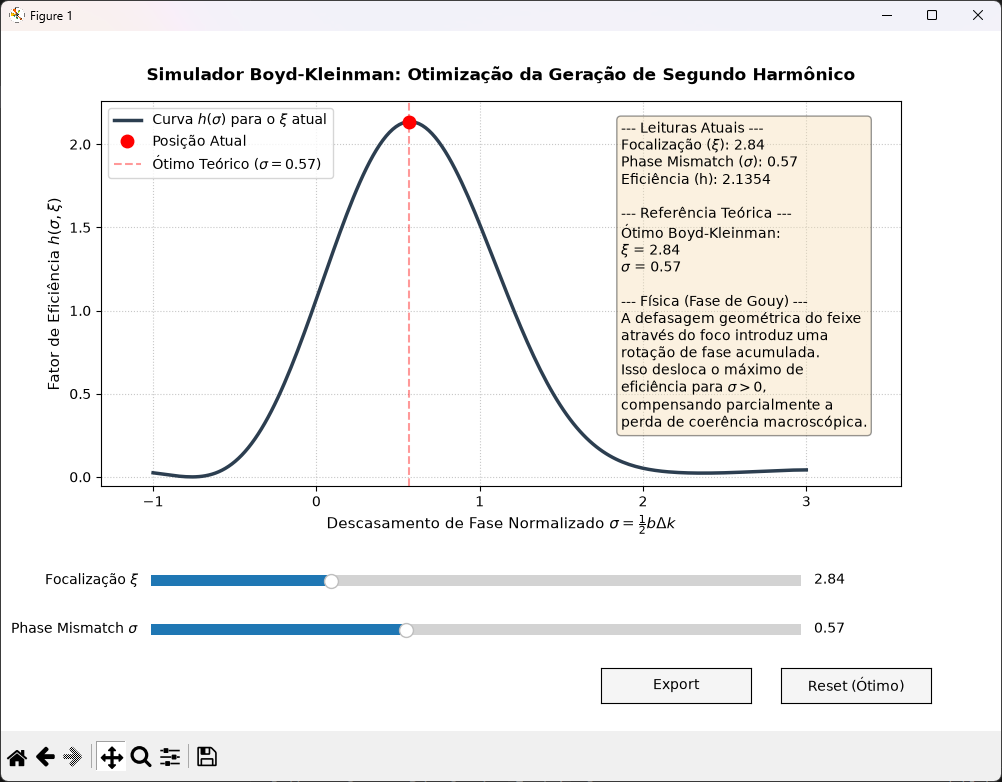
\includegraphics[width=0.75\columnwidth]{Interactive Boyd-Kleinman Simulator.png}
            \caption{Graphical User Interface (GUI) of the interactive script, developed to explore the influence of the Gouy phase shift on second-harmonic generation in real time.}
            \label{fig:simulator_gui}
        \end{figure}

        \begin{figure}[H]
            \centering
            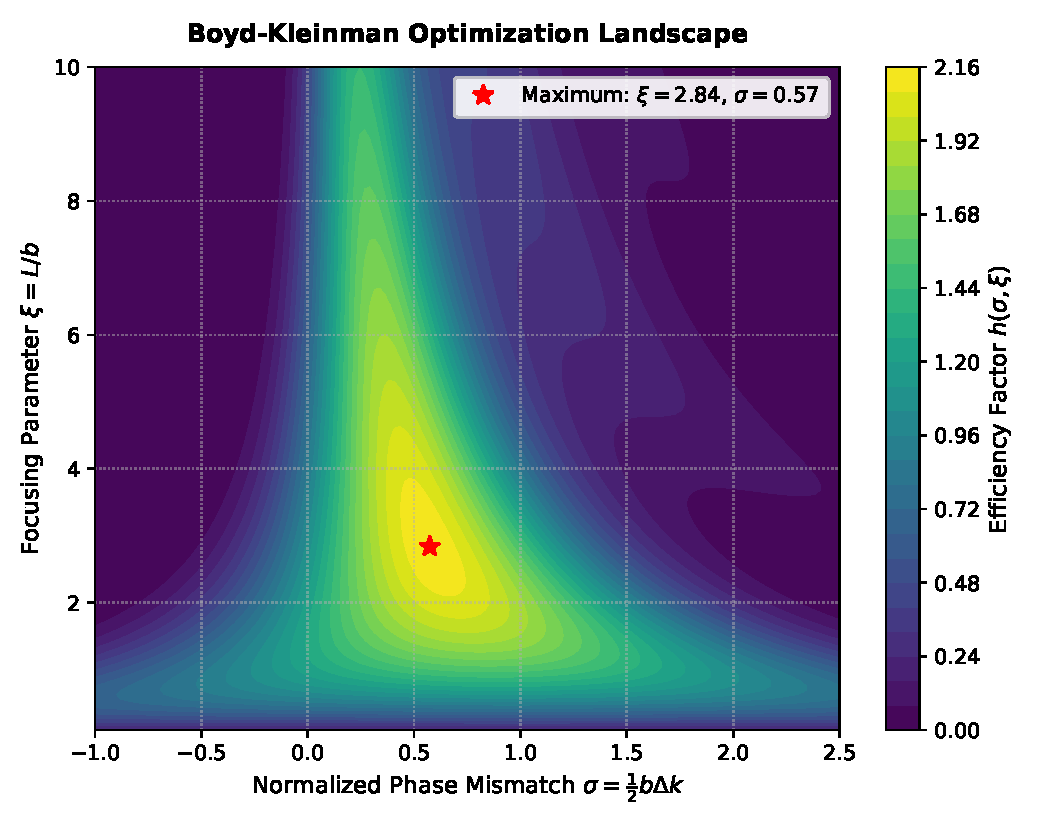
\includegraphics[width=\columnwidth]{boyd_kleinman_plot.pdf}
            \caption{Numerical evaluation of the Boyd-Kleinman factor $h(\sigma,\xi)$ as a function of the normalized phase mismatch $\sigma$ and focusing parameter $\xi$. The red star highlights the global optimum at $\xi \approx 2.84$ and $\sigma \approx 0.57$, where $h_{\max}\approx 1.068$.}
            \label{fig:boyd_kleinman}
        \end{figure}

\subsection*{(b) Phase Mismatch: Gaussian Beams vs. Plane Waves}

    The transition from the plane-wave regime to focused Gaussian beams introduces a fundamental shift in the phase-matching requirements. The reason is that a focused Gaussian beam is not merely a plane wave with finite transverse size: it has a longitudinally varying radius, a curved wavefront, and a Gouy phase. These features are described in Saleh and Teich, Sec.~3.1, especially Eqs.~(3.1-7)--(3.1-11) and the phase discussion around Eqs.~(3.1-23)--(3.1-24). In Boyd's nonlinear-optics treatment, the same physics enters through the denominator $(1+2iz/b)$ in Eq.~(2.10.11b), which modifies the longitudinal overlap integral relative to the plane-wave case.

    \paragraph*{Plane-Wave Limit}
        In the plane-wave limit, the beam is taken to have infinite transverse extent or, equivalently, a confocal parameter much larger than the nonlinear crystal length. In Boyd's notation this corresponds to the limit in which the denominator in Eq.~(2.10.11b) is approximately constant over the crystal. Boyd explicitly states this reduction in Eq.~(2.10.12a), obtaining
        \begin{equation}
            J_q(\Delta k,z_0,z)
            =
            \int_{z_0}^{z}
            e^{i\Delta k z'}dz'
            =
            \frac{
            e^{i\Delta k z}-e^{i\Delta k z_0}
            }{
            i\Delta k
            }.
            \label{eq:plane_wave_overlap}
        \end{equation}
        For an interaction length $L=z-z_0$, Boyd's Eq.~(2.10.12b) gives
        \begin{equation}
            |J_q|^2
            =
            L^2
            \operatorname{sinc}^2
            \left(
            \frac{\Delta k L}{2}
            \right).
            \label{eq:sinc_plane_wave}
        \end{equation}
        This is the usual plane-wave phase-matching factor. It reaches its maximum at
        \begin{equation}
            \Delta k=0.
        \end{equation}
        The same plane-wave SHG phase mismatch is defined in Boyd's Eq.~(2.7.12),
        \begin{equation}
            \Delta k = 2k_1-k_2,
        \end{equation}
        after the coupled-amplitude equation for the second-harmonic field in Eq.~(2.7.11). Thus, for plane waves, the mathematical and physical condition for maximum coherent buildup is simply perfect material phase matching.

    \paragraph*{The Role of the Gouy Phase Shift}
        For focused Gaussian beams, this conclusion is modified. The numerical result in Eq.~\eqref{eq:bk_optimum_sigma_xi} shows that the optimum mismatch shifts to
        \begin{equation}
            \sigma_{\mathrm{opt}}\approx 0.57,
        \end{equation}
        which implies a strictly nonzero material phase mismatch:
        \begin{equation}
            \Delta k_{\mathrm{opt}}
            =
            \frac{2\sigma_{\mathrm{opt}}}{b}
            >
            0.
        \end{equation}

        The physical origin of this shift is the Gouy phase. Saleh and Teich write the Gaussian beam phase in Eq.~(3.1-23) as containing, on axis, the term
        \begin{equation}
            \phi(0,z)=kz-\zeta_G(z),
        \end{equation}
        where, using the notation $\zeta_G$ to avoid confusion with Boyd's dimensionless coordinate,
        \begin{equation}
            \zeta_G(z)
            =
            \tan^{-1}
            \left(
            \frac{z}{z_R}
            \right).
        \end{equation}
        In Saleh and Teich's notation this function is denoted by $C(z)$ in Eq.~(3.1-10), with $z_0$ playing the role of the Rayleigh range. As the beam passes from $z=-\infty$ to $z=+\infty$, $\zeta_G(z)$ changes from $-\pi/2$ to $+\pi/2$, so the total Gouy phase change is $\pi$.

        In the nonlinear interaction, however, the source of the second-harmonic wave is not the fundamental field itself, but the nonlinear polarization
        \begin{equation}
            P_{\mathrm{NL}}(2\omega)\propto E_\omega^2.
        \end{equation}
        Therefore, if the fundamental field carries a Gouy phase contribution $\zeta_G(z)$, the nonlinear polarization driving SHG carries twice this contribution. This is exactly the qualitative point made by Boyd after Fig.~2.10.4: for $q$-th harmonic generation, the nonlinear polarization contains $A_1^q$ and therefore acquires a phase shift $q$ times larger than that of the incident fundamental field.

        If the material were perfectly phase matched in the plane-wave sense, $\Delta k=0$, the generated second-harmonic field and the nonlinear polarization would not remain optimally phased throughout the focal region. The geometric phase evolution associated with focusing would introduce a longitudinal phase slip. In a macroscopic crystal, contributions generated before and after the focus would then interfere less constructively, reducing the net SHG output.

        A positive wavevector mismatch compensates this geometric phase slip. In the notation used here, this means choosing
        \begin{equation}
            \Delta k>0,
        \end{equation}
        or, equivalently,
        \begin{equation}
            \sigma>0.
        \end{equation}
        This explains why the focused-beam optimum is not located at $\Delta k=0$, but instead at
        \begin{equation}
            \Delta k_{\mathrm{opt}}\approx \frac{3.2}{L}.
        \end{equation}
        The bulk material mismatch supplies a linear phase variation that compensates the nonlinear Gouy phase accumulated near the beam waist.

        Therefore, the focused Gaussian-beam problem differs from the plane-wave problem in two coupled ways:
        \begin{enumerate}
            \item the transverse confinement increases the intensity and therefore tends to increase the nonlinear conversion;
            \item the same confinement introduces diffraction and Gouy-phase effects, which modify the longitudinal phase-matching condition.
        \end{enumerate}
        The Boyd-Kleinman criterion is precisely the optimization of this trade-off. It selects the focusing parameter $\xi=L/b$ and the normalized mismatch $\sigma=b\Delta k/2$ that maximize the full Gaussian overlap integral, rather than the plane-wave $\operatorname{sinc}^2(\Delta kL/2)$ factor.

\end{resolucao}

        %\onecolumn
        
        \newpage
        % ============================================================================
% ex2.tex
% ============================================================================
% Exercício individual da lista.
% Este arquivo deve conter apenas o conteúdo do exercício e, quando desejado,
% sua resolução. Não deve carregar pacotes nem redefinir configurações globais.
%
% Interface adotada neste exemplo:
% - ambiente `exercicio` com identificador textual livre;
% - ambiente `resolucao` para a solução;
% - subseções internas apenas para organizar a exposição.
% ============================================================================

\begin{exercicio}[Problem 2 --- Paraxial Wave Equation in Cylindrical Coordinates]
Solve the paraxial wave equation in cylindrical coordinates, and show that the solutions are the Laguerre-Gaussian modes.
\end{exercicio}

\begin{resolucao}[Solution]

```
\subsection*{1. Derivation of the Paraxial Wave Equation (PWE)}

    We start from the linear, monochromatic Helmholtz equation for a scalar optical field $U(\mathbf{r})$ propagating in a homogeneous medium with wavevector $k$:
    \begin{equation}
        \nabla^2 U(\mathbf{r}) + k^2 U(\mathbf{r}) = 0.
        \label{eq:helmholtz}
    \end{equation}
    This is the scalar version of the homogeneous wave equation used for beam propagation in a source-free, linear medium. In \textbf{Section 3.1 of \authorlinkcite{Saleh}} (\textit{The Gaussian Beam}, pp.~80--88), Saleh and Teich introduce paraxial waves by writing the monochromatic complex amplitude as a rapidly oscillating axial carrier multiplied by a slowly varying envelope. Their convention is
    \begin{equation}
        U(\mathbf{r}) = A(\mathbf{r})e^{-jkz},
        \tag{Saleh Eq.~3.1-1}
    \end{equation}
    which leads to the paraxial Helmholtz equation given in their Eq.~(3.1-2). In this solution I use the equivalent carrier convention
    \begin{equation}
        U(\rho,\phi,z) = A(\rho,\phi,z)e^{ikz}.
        \label{eq:envelope_separation}
    \end{equation}
    The difference between the two conventions is only a global complex-conjugation/sign convention for the phase. With the convention in Eq.~\eqref{eq:envelope_separation}, the sign of the first-order longitudinal derivative in the paraxial equation is the one written below. The physical mode family is, of course, the same.
    
    To substitute Eq.~\eqref{eq:envelope_separation} into Eq.~\eqref{eq:helmholtz}, we evaluate the Laplacian operator. Since the desired modes are cylindrically symmetric up to an azimuthal phase factor, it is natural to use cylindrical coordinates:
    \begin{equation}
        \nabla^2
        =
        \nabla_T^2
        +
        \frac{\partial^2}{\partial z^2},
        \qquad
        \nabla_T^2
        =
        \frac{\partial^2}{\partial \rho^2}
        +
        \frac{1}{\rho}
        \frac{\partial}{\partial \rho}
        +
        \frac{1}{\rho^2}
        \frac{\partial^2}{\partial \phi^2}.
        \label{eq:laplacian_cylindrical}
    \end{equation}
    This is the same transverse-Laplacian structure used by \textbf{\authorlinkcite{Boyd}} in Sec.~2.10.1, where Boyd writes the paraxial wave equation for focused nonlinear-optics problems and gives the cylindrical form
    \[
        \nabla_T^2
        =
        \frac{1}{r}
        \frac{\partial}{\partial r}
        \left(
            r\frac{\partial}{\partial r}
        \right)
        +
        \frac{1}{r^2}
        \frac{\partial^2}{\partial\phi^2}.
    \]
    In the notation used here, $r$ is denoted by $\rho$.

    Let us explicitly calculate the first and second partial derivatives of the field $U$ with respect to the propagation coordinate $z$:
    \begin{equation}
        \frac{\partial U}{\partial z}
        =
        \left(
            \frac{\partial A}{\partial z}
            +
            ikA
        \right)e^{ikz},
        \label{eq:first_z_derivative}
    \end{equation}
    and
    \begin{equation}
        \frac{\partial^2 U}{\partial z^2}
        =
        \frac{\partial}{\partial z}
        \left[
            \left(
                \frac{\partial A}{\partial z}
                +
                ikA
            \right)e^{ikz}
        \right]
        =
        \left(
            \frac{\partial^2 A}{\partial z^2}
            +
            i2k\frac{\partial A}{\partial z}
            -
            k^2A
        \right)e^{ikz}.
        \label{eq:z_derivatives}
    \end{equation}
    
    Substituting Eq.~\eqref{eq:z_derivatives} into the Helmholtz equation \eqref{eq:helmholtz}, and using the fact that transverse derivatives act only on the envelope $A$, gives
    \begin{equation}
        \left(
            \nabla_T^2 A
            +
            \frac{\partial^2 A}{\partial z^2}
            +
            i2k\frac{\partial A}{\partial z}
            -
            k^2A
        \right)e^{ikz}
        +
        k^2Ae^{ikz}
        =
        0.
    \end{equation}
    The terms proportional to $k^2A$ cancel exactly, leaving
    \begin{equation}
        \nabla_T^2 A
        +
        \frac{\partial^2 A}{\partial z^2}
        +
        i2k\frac{\partial A}{\partial z}
        =
        0.
        \label{eq:exact_envelope_equation_before_paraxial}
    \end{equation}
    
    At this stage, we invoke the \textbf{paraxial approximation}. The physical assumption, also stated by Boyd in Sec.~2.10.1 when deriving his Eq.~(2.10.3), is that the envelope changes appreciably only over distances much larger than the optical wavelength. Thus the second derivative of the envelope with respect to $z$ is small compared with the first derivative multiplied by $k$:
    \begin{equation}
        \left|
            \frac{\partial^2 A}{\partial z^2}
        \right|
        \ll
        2k
        \left|
            \frac{\partial A}{\partial z}
        \right|.
        \label{eq:paraxial_approximation}
    \end{equation}
    Dropping $\partial^2 A/\partial z^2$ in Eq.~\eqref{eq:exact_envelope_equation_before_paraxial} gives the homogeneous paraxial wave equation:
    \begin{equation}
        \nabla_T^2 A
        +
        i2k
        \frac{\partial A}{\partial z}
        =
        0.
        \label{eq:pwe_compact}
    \end{equation}
    Written explicitly in cylindrical coordinates, Eq.~\eqref{eq:pwe_compact} becomes
    \begin{equation}
        \frac{\partial^2 A}{\partial \rho^2}
        +
        \frac{1}{\rho}
        \frac{\partial A}{\partial \rho}
        +
        \frac{1}{\rho^2}
        \frac{\partial^2 A}{\partial \phi^2}
        +
        i2k
        \frac{\partial A}{\partial z}
        =
        0.
        \label{eq:pwe_cyl_final}
    \end{equation}
    This is the cylindrical version of the paraxial Helmholtz equation used in \authorlinkcite{Saleh}, Sec.~3.1, Eq.~(3.1-2), after adapting the phase convention from $e^{-jkz}$ to $e^{ikz}$.

\subsection*{2. Azimuthal Separation of Variables}

    Because Eq.~\eqref{eq:pwe_cyl_final} is invariant under rotations around the $z$-axis, its solutions can be chosen as eigenfunctions of the azimuthal operator $-i\partial/\partial\phi$. This is the cylindrical-coordinate analogue of the separation procedure used by Saleh and Teich in Sec.~3.3 for Hermite-Gaussian beams, where the Cartesian transverse variables are separated. In Sec.~3.4, Saleh and Teich state that the Laguerre-Gaussian family is obtained by writing the paraxial Helmholtz equation in cylindrical coordinates $(\rho,\phi,z)$ and then separating variables in $\rho$ and $\phi$.

    We therefore seek solutions of the form
    \begin{equation}
        A(\rho,\phi,z)
        =
        u(\rho,z)e^{-il\phi},
        \qquad
        l\in\mathbb{Z}.
        \label{eq:azimuthal_sep}
    \end{equation}
    The integer $l$ labels the azimuthal phase winding. Its sign fixes the handedness of the helical phase; its magnitude $|l|$ controls the radial behavior near the beam axis.

    The second derivative with respect to $\phi$ is
    \begin{equation}
        \frac{\partial^2 A}{\partial \phi^2}
        =
        (-il)^2u(\rho,z)e^{-il\phi}
        =
        -l^2u(\rho,z)e^{-il\phi}.
    \end{equation}
    Substituting this into Eq.~\eqref{eq:pwe_cyl_final} and factoring out $e^{-il\phi}$ gives the radial paraxial equation
    \begin{equation}
        \frac{\partial^2 u}{\partial \rho^2}
        +
        \frac{1}{\rho}
        \frac{\partial u}{\partial \rho}
        -
        \frac{l^2}{\rho^2}u
        +
        i2k
        \frac{\partial u}{\partial z}
        =
        0.
        \label{eq:radial_pwe_step}
    \end{equation}

    A useful point appears already in Eq.~\eqref{eq:radial_pwe_step}. Near the beam axis, the singular term $-l^2u/\rho^2$ must be balanced by the radial derivatives. If the less singular terms are neglected locally near $\rho=0$, the leading radial equation is
    \begin{equation}
        \frac{d^2u}{d\rho^2}
        +
        \frac{1}{\rho}
        \frac{du}{d\rho}
        -
        \frac{l^2}{\rho^2}u
        \approx
        0.
    \end{equation}
    Seeking $u\sim \rho^\alpha$ gives
    \begin{equation}
        \alpha(\alpha-1)\rho^{\alpha-2}
        +
        \alpha\rho^{\alpha-2}
        -
        l^2\rho^{\alpha-2}
        =
        0,
    \end{equation}
    hence
    \begin{equation}
        \alpha^2-l^2=0
        \qquad\Rightarrow\qquad
        \alpha=\pm |l|.
    \end{equation}
    The solution proportional to $\rho^{-|l|}$ is singular at $\rho=0$ and is not physically acceptable for a finite-power beam. Therefore, a regular Laguerre-Gaussian mode with $l\neq 0$ must contain the factor
    \begin{equation}
        u(\rho,z)\propto \rho^{|l|}
        \quad
        \text{near}
        \quad
        \rho=0.
        \label{eq:near_axis_behavior}
    \end{equation}
    This is the main correction to the more naive ansatz in which the whole radial dependence is placed in an arbitrary function $R(x)$: the factor $\rho^{|l|}$ should be extracted explicitly, otherwise the singular centrifugal-like term $-l^2u/\rho^2$ is not handled cleanly.

\subsection*{3. Gaussian Envelope and Corrected Laguerre-Gaussian Ansatz}

    The fundamental Gaussian beam is the lowest-order solution of the paraxial equation. In Saleh and Teich, Sec.~3.1, the Gaussian beam is written in Eq.~(3.1-7) in terms of the beam radius $W(z)$, radius of curvature $R(z)$, Gouy phase $C(z)$, and Rayleigh range $z_0$, defined in Eqs.~(3.1-8)--(3.1-11). Using the more common notation
    \[
        W(z)\to w(z),
        \qquad
        z_0\to z_R,
        \qquad
        C(z)\to \zeta_G(z),
    \]
    these functions are
    \begin{equation}
        w(z)
        =
        w_0
        \sqrt{
            1+\left(\frac{z}{z_R}\right)^2
        },
        \label{eq:wz}
    \end{equation}
    \begin{equation}
        R(z)
        =
        z
        \left[
            1+
            \left(
                \frac{z_R}{z}
            \right)^2
        \right],
        \label{eq:Rz}
    \end{equation}
    \begin{equation}
        \zeta_G(z)
        =
        \tan^{-1}
        \left(
            \frac{z}{z_R}
        \right),
        \label{eq:gouy}
    \end{equation}
    and
    \begin{equation}
        z_R
        =
        \frac{\pi n w_0^2}{\lambda_0}
        =
        \frac{k w_0^2}{2},
        \label{eq:rayleigh_range}
    \end{equation}
    where $\lambda_0$ is the vacuum wavelength and $k=2\pi n/\lambda_0$ is the wavenumber in the medium.

    With the phase convention adopted in Eq.~\eqref{eq:envelope_separation}, a convenient fundamental Gaussian envelope is
    \begin{equation}
        \psi_0(\rho,z)
        =
        \frac{w_0}{w(z)}
        \exp\left[
            -\frac{\rho^2}{w^2(z)}
        \right]
        \exp\left[
            -i\frac{k\rho^2}{2R(z)}
        \right]
        \exp\left[
            i\zeta_G(z)
        \right].
        \label{eq:fundamental_gaussian_envelope}
    \end{equation}
    This is the same physical Gaussian beam as Saleh's Eq.~(3.1-7), with the phase signs adapted to the carrier convention used here.

    To construct higher-order modes in cylindrical coordinates, introduce the dimensionless radial variable
    \begin{equation}
        x
        =
        \frac{2\rho^2}{w^2(z)}.
        \label{eq:x_definition}
    \end{equation}
    The factor $\exp[-\rho^2/w^2(z)]$ in Eq.~\eqref{eq:fundamental_gaussian_envelope} is then $\exp(-x/2)$.

    Guided by the near-axis condition in Eq.~\eqref{eq:near_axis_behavior}, the correct radial ansatz should not be merely $R(x)\psi_0$. Instead, we write
    \begin{equation}
        u(\rho,z)
        =
        x^{|l|/2}
        F(x)
        \psi_0(\rho,z)
        \exp\left[
            i\Delta\zeta_{p,l}(z)
        \right],
        \label{eq:corrected_ansatz_before_phase}
    \end{equation}
    where $F(x)$ is a dimensionless radial function to be determined and $\Delta\zeta_{p,l}(z)$ is the additional Gouy phase beyond the fundamental Gaussian phase already contained in $\psi_0$.

    Since $x^{|l|/2}\propto \rho^{|l|}$, Eq.~\eqref{eq:corrected_ansatz_before_phase} automatically satisfies the required regularity condition at the beam axis. This is precisely the radial structure that appears in Saleh's Eq.~(3.4-1), where the Laguerre-Gaussian mode contains a factor proportional to
    \[
        \left(
            \frac{\rho}{W(z)}
        \right)^l
    \]
    in the notation of Saleh and Teich. In the present notation, allowing both handednesses of the azimuthal phase, this factor becomes
    \[
        \left(
            \frac{\sqrt{2}\rho}{w(z)}
        \right)^{|l|}.
    \]

\subsection*{4. Reduction to the Associated Laguerre Equation}

    We now substitute the corrected ansatz into the radial paraxial equation. It is useful to isolate the non-Gaussian radial factor
    \begin{equation}
        S(x)
        =
        x^{s/2}F(x),
        \qquad
        s=|l|.
        \label{eq:S_definition}
    \end{equation}
    Then
    \begin{equation}
        u(\rho,z)
        =
        S(x)\psi_0(\rho,z)
        \exp[
            i\Delta\zeta_{p,l}(z)
        ].
        \label{eq:u_with_S}
    \end{equation}

    The chain rule gives
    \begin{equation}
        \frac{\partial x}{\partial \rho}
        =
        \frac{4\rho}{w^2(z)},
        \qquad
        \frac{\partial^2 x}{\partial \rho^2}
        =
        \frac{4}{w^2(z)}.
        \label{eq:x_rho_derivatives}
    \end{equation}
    Therefore,
    \begin{equation}
        \frac{\partial S}{\partial \rho}
        =
        \frac{dS}{dx}
        \frac{\partial x}{\partial \rho}
        =
        \frac{4\rho}{w^2(z)}
        \frac{dS}{dx},
        \label{eq:first_chain_S}
    \end{equation}
    and
    \begin{equation}
        \frac{\partial^2 S}{\partial \rho^2}
        =
        \frac{4}{w^2(z)}
        \frac{dS}{dx}
        +
        \frac{16\rho^2}{w^4(z)}
        \frac{d^2S}{dx^2}
        =
        \frac{4}{w^2(z)}
        \frac{dS}{dx}
        +
        \frac{8x}{w^2(z)}
        \frac{d^2S}{dx^2}.
        \label{eq:second_chain_S}
    \end{equation}
    Since
    \begin{equation}
        S(x)=x^{s/2}F(x),
    \end{equation}
    its first two derivatives are
    \begin{equation}
        \frac{dS}{dx}
        =
        x^{s/2}\frac{dF}{dx}
        +
        \frac{s}{2}
        x^{s/2-1}F,
        \label{eq:S_first_derivative}
    \end{equation}
    and
    \begin{equation}
        \frac{d^2S}{dx^2}
        =
        x^{s/2}\frac{d^2F}{dx^2}
        +
        s x^{s/2-1}\frac{dF}{dx}
        +
        \frac{s}{2}
        \left(
            \frac{s}{2}-1
        \right)
        x^{s/2-2}F.
        \label{eq:S_second_derivative}
    \end{equation}

    Substitution of Eq.~\eqref{eq:u_with_S} into Eq.~\eqref{eq:radial_pwe_step} is algebraically long, but the structure is simple. The fundamental Gaussian factor $\psi_0(\rho,z)$ independently satisfies the paraxial equation. Hence all terms that would already be present for the fundamental mode cancel. The remaining terms are those generated by the radial modulation $S(x)$, by the azimuthal term $-l^2u/\rho^2$, and by the additional Gouy phase $\Delta\zeta_{p,l}(z)$.

    The reason for extracting $x^{s/2}$ is now visible: the terms proportional to $x^{s/2-1}F$ generated by differentiating $x^{s/2}$ cancel the singular contribution coming from
    \[
        -\frac{l^2}{\rho^2}u.
    \]
    After this cancellation, the differential equation for $F(x)$ becomes
    \begin{equation}
        x\frac{d^2F}{dx^2}
        +
        (s+1-x)
        \frac{dF}{dx}
        +
        \Lambda F
        =
        0,
        \qquad
        s=|l|,
        \label{eq:laguerre_with_lambda}
    \end{equation}
    where $\Lambda$ is the separation constant associated with the additional longitudinal phase. More explicitly, consistency of the $z$-dependent terms gives
    \begin{equation}
        \frac{d\Delta\zeta_{p,l}}{dz}
        =
        (2\Lambda+s)
        \frac{d\zeta_G}{dz}.
        \label{eq:extra_gouy_relation_lambda}
    \end{equation}
    The physical finite-power solutions occur when the radial series terminates. This requires
    \begin{equation}
        \Lambda=p,
        \qquad
        p=0,1,2,\ldots.
        \label{eq:p_integer_condition}
    \end{equation}
    With this identification, Eq.~\eqref{eq:laguerre_with_lambda} becomes
    \begin{equation}
        \boxed{
        x\frac{d^2F}{dx^2}
        +
        (|l|+1-x)
        \frac{dF}{dx}
        +
        pF
        =
        0
        }.
        \label{eq:associated_laguerre_final}
    \end{equation}
    This is the associated Laguerre differential equation. Therefore,
    \begin{equation}
        F(x)
        =
        L_p^{|l|}(x),
        \label{eq:laguerre_solution}
    \end{equation}
    where $L_p^{|l|}$ is an associated Laguerre polynomial.

    The normalizability condition is important. If $p$ were not a non-negative integer, the solution would not terminate into a polynomial and the radial factor would generally grow too rapidly at large $x$ to represent a finite-power beam after multiplication by the Gaussian envelope. The physically acceptable paraxial modes therefore select the discrete radial index
    \[
        p=0,1,2,\ldots.
    \]

\subsection*{5. Determination of the Generalized Gouy Phase}

    Saleh and Teich's Gaussian beam has a Gouy phase $C(z)$, given in their Eq.~(3.1-10). In the notation used here,
    \[
        C(z)\equiv \zeta_G(z)
        =
        \tan^{-1}
        \left(
            \frac{z}{z_R}
        \right).
    \]
    Differentiating gives
    \begin{equation}
        \frac{d\zeta_G}{dz}
        =
        \frac{1}{z_R}
        \frac{1}{1+(z/z_R)^2}.
        \label{eq:gouy_derivative_1}
    \end{equation}
    Using
    \[
        w^2(z)
        =
        w_0^2
        \left[
            1+
            \left(
                \frac{z}{z_R}
            \right)^2
        \right],
        \qquad
        k w_0^2 = 2z_R,
    \]
    Eq.~\eqref{eq:gouy_derivative_1} may also be written as
    \begin{equation}
        \frac{d\zeta_G}{dz}
        =
        \frac{2}{k w^2(z)}.
        \label{eq:gouy_derivative_2}
    \end{equation}

    From Eq.~\eqref{eq:extra_gouy_relation_lambda} with $\Lambda=p$, the additional Gouy phase beyond the fundamental Gaussian contribution is
    \begin{equation}
        \frac{d\Delta\zeta_{p,l}}{dz}
        =
        (2p+|l|)
        \frac{d\zeta_G}{dz}.
        \label{eq:extra_gouy_differential}
    \end{equation}
    Integrating from the waist plane $z=0$, where $\zeta_G(0)=0$, gives
    \begin{equation}
        \Delta\zeta_{p,l}(z)
        =
        (2p+|l|)
        \zeta_G(z)
        =
        (2p+|l|)
        \tan^{-1}
        \left(
            \frac{z}{z_R}
        \right).
        \label{eq:extra_gouy_integrated}
    \end{equation}
    The total Gouy phase of the mode is the fundamental Gaussian Gouy phase already contained in $\psi_0$ plus this excess phase:
    \begin{equation}
        \boxed{
        \zeta_{p,l}^{\mathrm{tot}}(z)
        =
        (2p+|l|+1)
        \tan^{-1}
        \left(
            \frac{z}{z_R}
        \right)
        }.
        \label{eq:total_gouy_lg}
    \end{equation}
    This is the corrected form of the result. It agrees with Saleh and Teich's Eq.~(3.4-1), where the Gouy phase factor is written as $(l+2m+1)C(z)$, with $l\geq0$ denoting the azimuthal index magnitude and $m\geq0$ the radial index. In the notation of this solution,
    \[
        m \leftrightarrow p,
        \qquad
        l_{\mathrm{Saleh}}\leftrightarrow |l|.
    \]
    Therefore,
    \[
        l_{\mathrm{Saleh}}+2m+1
        =
        |l|+2p+1.
    \]

\subsection*{6. Final Laguerre-Gaussian Modes}

    Combining the Gaussian envelope, the regular near-axis radial factor, the associated Laguerre polynomial, the helical azimuthal phase, and the generalized Gouy phase, we obtain
    \begin{equation}
        \boxed{
        \begin{aligned}
        A_{p,l}(\rho,\phi,z)
        &=
        A_{p,l}^{(0)}
        \frac{w_0}{w(z)}
        \left(
            \frac{\sqrt{2}\rho}{w(z)}
        \right)^{|l|}
        L_p^{|l|}
        \left(
            \frac{2\rho^2}{w^2(z)}
        \right)
        \exp\left[
            -\frac{\rho^2}{w^2(z)}
        \right]
        \\[4pt]
        &\quad\times
        \exp\left[
            -i\frac{k\rho^2}{2R(z)}
        \right]
        \exp\left[
            i(2p+|l|+1)
            \zeta_G(z)
        \right]
        \exp(-il\phi).
        \end{aligned}
        }
        \label{eq:LG_final}
    \end{equation}
    Here
    \[
        p=0,1,2,\ldots,
        \qquad
        l\in\mathbb{Z}.
    \]
    The radial index $p$ counts the number of radial nodes, while the azimuthal index $l$ determines the helical phase structure and the orbital angular momentum content of the mode. The magnitude $|l|$ determines the strength of the central intensity null: for $l\neq0$, the factor $\rho^{|l|}$ forces the field to vanish on the beam axis.

    The associated physical optical field is then
    \begin{equation}
        U_{p,l}(\rho,\phi,z)
        =
        A_{p,l}(\rho,\phi,z)e^{ikz},
        \label{eq:LG_total_field}
    \end{equation}
    using the carrier convention adopted in Eq.~\eqref{eq:envelope_separation}. If one instead uses Saleh and Teich's carrier convention $e^{-jkz}$, the corresponding phase signs in Eq.~\eqref{eq:LG_final} are complex conjugated, but the intensity profile, Gouy-phase order, mode indices, and physical content are unchanged.

    Thus, the paraxial wave equation in cylindrical coordinates admits a complete family of finite-power beam-like solutions of the form
    \[
        LG_p^l,
    \]
    namely the Laguerre-Gaussian modes. This is the cylindrical counterpart of the Hermite-Gaussian family obtained by separating the same paraxial Helmholtz equation in Cartesian coordinates. As stated in Saleh and Teich, Sec.~3.4, the Laguerre-Gaussian modes form an alternate complete set of solutions to the paraxial Helmholtz equation.
```

\end{resolucao}

        
        \newpage
        % ============================================================================
% ex3.tex
% ============================================================================
% Exercício individual da lista.
% Este arquivo deve conter apenas o conteúdo do exercício e, quando desejado,
% sua resolução. Não deve carregar pacotes nem redefinir configurações globais.
%
% Interface adotada neste exemplo:
% - ambiente "exercicio" com identificador textual livre;
% - ambiente "resolucao" para a solução;
% - subseções internas apenas para organizar a exposição.
% ============================================================================

\begin{exercicio}[Problem 3 --- Hermite-Gaussian and Laguerre-Gaussian Transformation]
Show that the transformation between Hermite-Gaussian modes and Laguerre-Gaussian modes is block-diagonal, i.e., that any Hermite-Gaussian mode of order $N$ is a superposition of Laguerre-Gaussian modes with the same order.
\end{exercicio}

% Para mudar o título, basta alterar o texto entre colchetes []
% Ex: [Resolução] ou [Solution]

\begin{resolucao}[Solution]

To prove that the transformation matrix connecting the Hermite-Gaussian (HG) and Laguerre-Gaussian (LG) bases is block-diagonal, we must demonstrate that a mode from one basis can only project onto modes from the other basis if both modes share the same total transverse order $N$.

The relevant mathematical structure comes from \textbf{Chapter 3 of \authorlinkcite{Saleh}}, especially Sections~3.3 and~3.4. In Sec.~3.3, Saleh and Teich derive the Hermite-Gaussian modes by separating the paraxial Helmholtz equation in Cartesian coordinates. Their Eq.~(3.3-10) gives the complex amplitude of the HG mode, and Eq.~(3.3-9) gives the excess Gouy phase proportional to the sum of the two Cartesian indices. In Sec.~3.4, they state that the Laguerre-Gaussian modes are obtained by writing the same paraxial Helmholtz equation in cylindrical coordinates and separating the variables $\rho$ and $\phi$; their Eq.~(3.4-1) gives the complex amplitude of the LG mode. The same structure also appears in \textbf{\authorlinkcite{Yariv}}, Sec.~6.9, Eq.~(6.9-1), where high-order Gaussian modes in homogeneous media carry a Gouy phase proportional to the total transverse order plus one.

Therefore, the proof below is based on two equivalent facts:
\begin{enumerate}
\item HG and LG modes solve the same paraxial wave equation, but in different transverse coordinate systems.
\item Both families acquire a Gouy phase determined only by the same total transverse order $N$.
\end{enumerate}

\subsection*{1. Definition of the Bases and the Total Mode Order}

```
Both the HG and LG modes form complete orthogonal basis sets for paraxial optical fields. Saleh and Teich state this explicitly at the beginning of Sec.~3.4: the Hermite-Gaussian beams form a complete set of solutions of the paraxial Helmholtz equation, and the Laguerre-Gaussian beams form an alternate complete set obtained in cylindrical coordinates.

\paragraph*{Hermite-Gaussian Modes}
The Hermite-Gaussian modes are separable in Cartesian coordinates $(x,y)$. In Saleh and Teich's notation, Eq.~(3.3-10) gives the complex amplitude of a mode labeled by two non-negative integers. In the notation used here, these indices are denoted by $(n,m)$:
\begin{equation}
    HG_{n,m},
    \qquad
    n,m=0,1,2,\ldots.
\end{equation}
The corresponding total transverse order is
\begin{equation}
    N_{\mathrm{HG}}=n+m.
    \label{eq:NHG_definition}
\end{equation}

Using the usual notation
\[
    W(z)\to w(z),
    \qquad
    C(z)\to \zeta(z),
    \qquad
    z_0\to z_R,
\]
and suppressing normalization constants, the Hermite-Gaussian field may be written as
\begin{equation}
    \begin{aligned}
    U_{n,m}^{\mathrm{HG}}(x,y,z)
    &\propto
    \frac{w_0}{w(z)}
    H_n\left(\frac{\sqrt{2}x}{w(z)}\right)
    H_m\left(\frac{\sqrt{2}y}{w(z)}\right)
    \exp\left[-\frac{x^2+y^2}{w^2(z)}\right]
    \\[3pt]
    &\quad\times
    \exp\left[-i\frac{k(x^2+y^2)}{2R(z)}\right]
    \exp\left[ikz\right]
    \exp\left[-i(n+m+1)\zeta(z)\right].
    \end{aligned}
    \label{eq:HG_mode_form}
\end{equation}
This expression is the same content as Saleh and Teich's Eq.~(3.3-10), up to the sign convention used for the carrier phase. The important point for this exercise is the Gouy phase:
\begin{equation}
    \Phi_{\mathrm{Gouy}}^{\mathrm{HG}}(z)
    =
    (n+m+1)\zeta(z)
    =
    (N_{\mathrm{HG}}+1)\zeta(z).
    \label{eq:HG_gouy_order}
\end{equation}
This follows directly from Saleh and Teich's Eq.~(3.3-9), where the excess phase is proportional to the sum of the two Cartesian indices.

\paragraph*{Laguerre-Gaussian Modes}
The Laguerre-Gaussian modes are separable in cylindrical coordinates $(\rho,\phi)$. In Saleh and Teich's notation, Eq.~(3.4-1) writes the LG mode with an azimuthal index and a radial index. In this solution, I use the standard notation
\begin{equation}
    LG_p^l,
    \qquad
    p=0,1,2,\ldots,
    \qquad
    l\in\mathbb{Z},
\end{equation}
where $p$ is the radial index and $l$ is the signed azimuthal, or topological, index. Since Saleh and Teich write the azimuthal index as a non-negative integer, their azimuthal index corresponds here to $|l|$.

The total transverse order of an LG mode is
\begin{equation}
    N_{\mathrm{LG}}=2p+|l|.
    \label{eq:NLG_definition}
\end{equation}
Again suppressing normalization constants, the corresponding field may be written as
\begin{equation}
    \begin{aligned}
    U_{p,l}^{\mathrm{LG}}(\rho,\phi,z)
    &\propto
    \frac{w_0}{w(z)}
    \left(
        \frac{\sqrt{2}\rho}{w(z)}
    \right)^{|l|}
    L_p^{|l|}
    \left(
        \frac{2\rho^2}{w^2(z)}
    \right)
    \exp\left[-\frac{\rho^2}{w^2(z)}\right]
    \\[3pt]
    &\quad\times
    \exp\left[-i\frac{k\rho^2}{2R(z)}\right]
    \exp(ikz)
    \exp\left[-i(2p+|l|+1)\zeta(z)\right]
    \exp(-il\phi).
    \end{aligned}
    \label{eq:LG_mode_form}
\end{equation}
This is the same mode structure as Saleh and Teich's Eq.~(3.4-1), rewritten with signed azimuthal index $l$. Saleh and Teich explicitly emphasize, after Eq.~(3.4-1), that the phase behavior of the LG beam has the same Gaussian-beam dependence as Eq.~(3.1-7), except that the Gouy phase is enhanced by the factor
\[
    |l|+2p+1.
\]
Hence
\begin{equation}
    \Phi_{\mathrm{Gouy}}^{\mathrm{LG}}(z)
    =
    (2p+|l|+1)\zeta(z)
    =
    (N_{\mathrm{LG}}+1)\zeta(z).
    \label{eq:LG_gouy_order}
\end{equation}

The key comparison is therefore
\begin{equation}
    \boxed{
    \Phi_{\mathrm{Gouy}}^{\mathrm{HG}}=(N_{\mathrm{HG}}+1)\zeta(z),
    \qquad
    \Phi_{\mathrm{Gouy}}^{\mathrm{LG}}=(N_{\mathrm{LG}}+1)\zeta(z)
    }.
    \label{eq:gouy_comparison}
\end{equation}
Both bases use the same propagation eigenvalue label $N$.
```

\subsection*{2. Physical Argument: Propagation and Gouy-Phase Invariance}

```
Since the Laguerre-Gaussian modes form a complete basis, any Hermite-Gaussian mode can be expanded in that basis at a fixed transverse plane. Let us write this expansion at the waist plane $z=0$, where $\zeta(0)=0$:
\begin{equation}
    U_{n,m}^{\mathrm{HG}}(x,y,0)
    =
    \sum_{p=0}^{\infty}
    \sum_{l=-\infty}^{\infty}
    c_{p,l}^{(n,m)}
    U_{p,l}^{\mathrm{LG}}(\rho,\phi,0).
    \label{eq:expansion_z0}
\end{equation}
The coefficients are the overlap amplitudes
\begin{equation}
    c_{p,l}^{(n,m)}
    =
    \left\langle
    LG_p^l
    \middle|
    HG_{n,m}
    \right\rangle
    =
    \int
    \left[
    U_{p,l}^{\mathrm{LG}}(\rho,\phi,0)
    \right]^*
    U_{n,m}^{\mathrm{HG}}(x,y,0)
    \,d^2\mathbf r_\perp.
    \label{eq:overlap_coefficients}
\end{equation}
Because the paraxial wave equation is linear, each mode in Eq.~\eqref{eq:expansion_z0} propagates independently. Therefore, after propagation to a general position $z$, each term acquires its own Gouy phase:
\begin{equation}
    U_{n,m}^{\mathrm{HG}}(x,y,z)
    =
    \sum_{p,l}
    c_{p,l}^{(n,m)}
    U_{p,l}^{\mathrm{LG}}(\rho,\phi,z).
    \label{eq:expansion_z}
\end{equation}

Now isolate only the Gouy-phase factors, since the plane-wave carrier $\exp(ikz)$, the Gaussian curvature factor, and the beam width scaling are common structures inside the paraxial Gaussian-mode family. Using Eqs.~\eqref{eq:HG_gouy_order} and~\eqref{eq:LG_gouy_order}, Eq.~\eqref{eq:expansion_z} contains terms of the form
\begin{equation}
    e^{-i(N_{\mathrm{HG}}+1)\zeta(z)}
    =
    \sum_{p,l}
    c_{p,l}^{(n,m)}
    \left(\text{transverse LG structure}\right)
    e^{-i(N_{\mathrm{LG}}+1)\zeta(z)}.
    \label{eq:gouy_phase_comparison_expansion}
\end{equation}
Multiplying both sides by $e^{+i(N_{\mathrm{HG}}+1)\zeta(z)}$, every LG contribution carries the relative phase
\begin{equation}
    \exp\left[
        -i
        (N_{\mathrm{LG}}-N_{\mathrm{HG}})
        \zeta(z)
    \right].
    \label{eq:relative_gouy_phase}
\end{equation}

The left-hand side represents one single HG propagation eigenmode. It does not contain longitudinal beating between different Gouy orders. If the right-hand side contained any term with
\[
    N_{\mathrm{LG}}\neq N_{\mathrm{HG}},
\]
then that term would acquire a relative phase depending on $z$ through Eq.~\eqref{eq:relative_gouy_phase}. Since $\zeta(z)=\tan^{-1}(z/z_R)$ varies continuously during propagation, this relative phase would generate longitudinal beating between different transverse orders.

Such beating cannot occur in the propagation of a single HG mode, because Eq.~(3.3-10) of Saleh and Teich shows that $HG_{n,m}$ is itself an exact propagation mode of the paraxial Helmholtz equation. Therefore, consistency for all $z$ requires
\begin{equation}
    c_{p,l}^{(n,m)}=0
    \qquad
    \text{whenever}
    \qquad
    2p+|l|\neq n+m.
    \label{eq:block_condition}
\end{equation}
This already proves the block-diagonal property:
\begin{equation}
    \boxed{
    \left\langle
    LG_p^l
    \middle|
    HG_{n,m}
    \right\rangle
    =
    0
    \quad
    \text{if}
    \quad
    2p+|l|\neq n+m.
    }
    \label{eq:overlap_selection_rule}
\end{equation}
```

\subsection*{3. Mathematical Argument: Degenerate Subspaces of the Two-Dimensional Harmonic Oscillator}

```
The same result can be seen algebraically at the waist plane. At $z=0$, all HG and LG modes contain the same fundamental Gaussian envelope. After this common Gaussian factor is removed, what remains is a polynomial structure.

To make this explicit, define the dimensionless Cartesian variables
\begin{equation}
    X=\frac{\sqrt{2}x}{w_0},
    \qquad
    Y=\frac{\sqrt{2}y}{w_0}.
    \label{eq:dimensionless_cartesian}
\end{equation}
Then the waist-plane HG mode has the structure
\begin{equation}
    HG_{n,m}(X,Y,0)
    \propto
    H_n(X)H_m(Y)
    \exp\left[
        -\frac{X^2+Y^2}{2}
    \right].
    \label{eq:HG_waist_polynomial}
\end{equation}
This is exactly the functional structure indicated by Saleh and Teich's Eq.~(3.3-11), where the Hermite-Gaussian function is a Hermite polynomial multiplied by a Gaussian.

Similarly, using
\begin{equation}
    \rho^2=x^2+y^2,
    \qquad
    e^{-il\phi}
    =
    \left(
        \frac{x-iy}{\rho}
    \right)^l
    \quad
    (l>0),
    \label{eq:polar_cartesian_relation}
\end{equation}
and the analogous expression for $l<0$, the azimuthal factor of an LG mode may be written as a Cartesian polynomial:
\begin{equation}
    \rho^{|l|}e^{-il\phi}
    =
    \begin{cases}
        (x-iy)^l, & l\geq 0,\\[4pt]
        (x+iy)^{|l|}, & l<0.
    \end{cases}
    \label{eq:azimuthal_polynomial}
\end{equation}
Therefore, the waist-plane LG mode has the polynomial structure
\begin{equation}
    LG_p^l(\rho,\phi,0)
    \propto
    \rho^{|l|}
    L_p^{|l|}
    \left(
        \frac{2\rho^2}{w_0^2}
    \right)
    e^{-il\phi}
    \exp\left[
        -\frac{\rho^2}{w_0^2}
    \right].
    \label{eq:LG_waist_polynomial}
\end{equation}
Since $L_p^{|l|}$ is a polynomial of degree $p$ in $\rho^2=x^2+y^2$, the highest total Cartesian degree of the LG polynomial part is
\begin{equation}
    |l|+2p=N_{\mathrm{LG}}.
    \label{eq:LG_polynomial_order}
\end{equation}

However, the statement is stronger than a simple comparison of polynomial degrees. The proper mathematical reason is that both the HG and LG waist-plane functions are eigenfunctions of the same two-dimensional harmonic-oscillator operator. In dimensionless variables, this operator may be written as
\begin{equation}
    \hat{N}
    =
    \frac{1}{2}
    \left(
        -\frac{\partial^2}{\partial X^2}
        -\frac{\partial^2}{\partial Y^2}
        +X^2+Y^2
    \right)
    -1.
    \label{eq:number_operator_2d}
\end{equation}
The Hermite-Gaussian functions diagonalize this operator in Cartesian coordinates:
\begin{equation}
    \hat{N}
    HG_{n,m}
    =
    (n+m)
    HG_{n,m}.
    \label{eq:HG_number_eigenvalue}
\end{equation}
The Laguerre-Gaussian functions diagonalize the same operator in polar coordinates:
\begin{equation}
    \hat{N}
    LG_p^l
    =
    (2p+|l|)
    LG_p^l.
    \label{eq:LG_number_eigenvalue}
\end{equation}
This is the optical version of the degeneracy of the two-dimensional isotropic harmonic oscillator: the same eigenspace of total excitation number $N$ may be described either by Cartesian quantum numbers $(n,m)$ or by polar quantum numbers $(p,l)$.

Since $\hat{N}$ is self-adjoint, eigenfunctions with different eigenvalues are orthogonal. Thus, if
\[
    n+m\neq 2p+|l|,
\]
then
\begin{equation}
    \left\langle
    LG_p^l
    \middle|
    HG_{n,m}
    \right\rangle
    =
    0.
    \label{eq:orthogonality_different_N}
\end{equation}
This is the same selection rule obtained from the Gouy-phase argument, but now written as an orthogonality relation between different eigenspaces of the transverse harmonic-oscillator operator.
```

\subsection*{4. Dimension of Each Block}

```
For a fixed total order $N$, the HG basis contains the $N+1$ modes
\begin{equation}
    HG_{0,N},
    HG_{1,N-1},
    HG_{2,N-2},
    \ldots,
    HG_{N,0}.
    \label{eq:HG_block_modes}
\end{equation}
Therefore, the HG subspace of order $N$ has dimension
\begin{equation}
    \dim \mathcal{H}_N^{\mathrm{HG}}=N+1.
    \label{eq:HG_block_dimension}
\end{equation}

The LG basis at the same order consists of all integer $l$ such that
\begin{equation}
    N=2p+|l|,
    \qquad
    p=0,1,2,\ldots.
    \label{eq:LG_order_constraint}
\end{equation}
Hence $|l|$ must have the same parity as $N$, and the allowed signed values are
\begin{equation}
    l=-N,\,-N+2,\,-N+4,\ldots,\,N-2,\,N.
    \label{eq:allowed_l_values}
\end{equation}
This gives exactly $N+1$ allowed LG modes. Therefore,
\begin{equation}
    \dim \mathcal{H}_N^{\mathrm{LG}}=N+1.
    \label{eq:LG_block_dimension}
\end{equation}

Since both bases span the same eigenspace of $\hat{N}$ with the same dimension, the transformation between them is unitary within each fixed-$N$ subspace and zero between different-$N$ subspaces.
```

\subsection*{5. Explicit Block-Diagonal Form}

```
Let us order the HG basis by increasing total order:
\begin{equation}
    \{HG_{0,0}\};
    \quad
    \{HG_{1,0},HG_{0,1}\};
    \quad
    \{HG_{2,0},HG_{1,1},HG_{0,2}\};
    \quad
    \ldots
\end{equation}
and order the LG basis similarly:
\begin{equation}
    \{LG_0^0\};
    \quad
    \{LG_0^{-1},LG_0^{+1}\};
    \quad
    \{LG_0^{-2},LG_1^0,LG_0^{+2}\};
    \quad
    \ldots.
\end{equation}

The transformation matrix
\begin{equation}
    M_{(p,l),(n,m)}
    =
    \left\langle
    LG_p^l
    \middle|
    HG_{n,m}
    \right\rangle
    \label{eq:transformation_matrix}
\end{equation}
then has the structure
\begin{equation}
    M
    =
    \begin{pmatrix}
        M^{(0)} & 0 & 0 & 0 & \cdots \\
        0 & M^{(1)} & 0 & 0 & \cdots \\
        0 & 0 & M^{(2)} & 0 & \cdots \\
        0 & 0 & 0 & M^{(3)} & \cdots \\
        \vdots & \vdots & \vdots & \vdots & \ddots
    \end{pmatrix},
    \label{eq:block_diagonal_matrix}
\end{equation}
where each block $M^{(N)}$ is an $(N+1)\times(N+1)$ matrix acting only inside the fixed-order subspace
\begin{equation}
    \mathcal H_N
    =
    \mathrm{span}
    \left\{
        HG_{n,m}: n+m=N
    \right\}
    =
    \mathrm{span}
    \left\{
        LG_p^l: 2p+|l|=N
    \right\}.
    \label{eq:same_subspace}
\end{equation}
```

\subsection*{6. Low-Order Examples}

```
The first few blocks illustrate the selection rule.

\paragraph*{Order $N=0$}
There is only one mode:
\begin{equation}
    HG_{0,0}
    \leftrightarrow
    LG_0^0.
\end{equation}
Both are simply the fundamental Gaussian beam, as stated by Saleh and Teich below Eq.~(3.4-1).

\paragraph*{Order $N=1$}
The HG basis is
\begin{equation}
    \{HG_{1,0},HG_{0,1}\},
\end{equation}
while the LG basis is
\begin{equation}
    \{LG_0^{+1},LG_0^{-1}\}.
\end{equation}
Up to normalization and phase conventions,
\begin{equation}
    LG_0^{+1}
    \propto
    HG_{1,0}
    -
    iHG_{0,1},
    \qquad
    LG_0^{-1}
    \propto
    HG_{1,0}
    +
    iHG_{0,1}.
    \label{eq:N1_example}
\end{equation}
This is the same type of result requested in Saleh and Teich's Exercise~3.4-1, where a first-order Laguerre-Gaussian beam is written as a superposition of first-order Hermite-Gaussian beams with a relative phase of $\pi/2$.

\paragraph*{Order $N=2$}
The HG basis is
\begin{equation}
    \{HG_{2,0},HG_{1,1},HG_{0,2}\},
\end{equation}
and the LG basis is
\begin{equation}
    \{LG_0^{+2},LG_1^0,LG_0^{-2}\}.
\end{equation}
Again, no modes of order $N=0$ or $N=1$ enter this expansion, because their Gouy phases and oscillator eigenvalues are different.
```

\subsection*{Conclusion}

```
The transformation between Hermite-Gaussian and Laguerre-Gaussian modes is block-diagonal because both families are complete bases of the same paraxial solution space, but they decompose that space into the same invariant subspaces labeled by the total transverse order
\begin{equation}
    N=n+m=2p+|l|.
\end{equation}
The physical reason is the Gouy phase: modes of different $N$ acquire different propagation phases $(N+1)\zeta(z)$ and therefore cannot mix in the expansion of a single propagation eigenmode. The mathematical reason is the degeneracy of the two-dimensional isotropic harmonic oscillator: HG modes diagonalize the transverse oscillator in Cartesian coordinates, while LG modes diagonalize the same oscillator in polar coordinates. Thus, the overlap matrix satisfies
\begin{equation}
    \boxed{
    \left\langle
    LG_p^l
    \middle|
    HG_{n,m}
    \right\rangle
    =
    0
    \quad
    \text{unless}
    \quad
    2p+|l|=n+m
    }.
\end{equation}
Therefore, when the modes are ordered by increasing $N$, the transformation matrix contains nonzero elements only inside finite-dimensional diagonal blocks of size $(N+1)\times(N+1)$.
```

\end{resolucao}

        
        \newpage
        % ============================================================================
% ex4.tex
% ============================================================================
% Exercício individual da lista.
% Este arquivo deve conter apenas o conteúdo do exercício e, quando desejado,
% sua resolução. Não deve carregar pacotes nem redefinir configurações globais.
%
% Interface adotada neste exemplo:
% - ambiente `exercicio` com identificador textual livre;
% - ambiente `resolucao` para a solução;
% - subseções internas apenas para organizar a exposição.
% ============================================================================

\begin{exercicio}[Problem 4 --- Resonance Frequencies of an Optical Resonator]
Consider an optical resonator with length $L$ and mirrors of curvature radii $R_{1}$ and $R_{2}$.

\begin{enumerate}[a)]
\item Show that the resonance frequencies are given by:
$[\nu_{mnq} = \frac{c}{2L} \left[ q + \frac{1}{\pi} (m+n+1) \arccos\left(\pm\sqrt{g_{1}g_{2}}\right) \right]]$,
where $g_{j} = 1 - L/R_{j}$ for $j=1,2$.
\item Discuss how the resonance frequencies of different spatial modes are separated according to the cavity geometry.
\end{enumerate}
\end{exercicio}

\begin{resolucao}[Solution]

\subsection*{(a) Derivation of the Resonance Frequencies}

    The starting point is the wave-optics treatment of spherical-mirror resonators in \textbf{Chapter 11 of \authorlinkcite{Saleh}}, specifically \textbf{Section 11.2, Spherical-Mirror Resonators}. Saleh and Teich first show that a Gaussian beam can be self-consistently fitted to a pair of spherical mirrors if the wavefront curvature of the Gaussian beam matches the mirror curvature at the mirror positions. This is developed in Sec.~11.2B using the Gaussian-beam parameters previously introduced in Sec.~3.1: the beam radius $W(z)$, the radius of curvature $R(z)$, and the Rayleigh range $z_0$, which appear again as Eqs.~(11.2-8)--(11.2-10).

    The resonance-frequency calculation then follows in Sec.~11.2C. Saleh and Teich use the Gaussian-beam phase from Eq.~(3.1-23) and rewrite it for the resonator geometry in Eq.~(11.2-25). For Hermite-Gaussian modes, the same argument is extended in Sec.~11.2D using the Gouy-phase dependence already obtained in Sec.~3.3, especially Eq.~(3.3-10). The final result for Hermite-Gaussian resonator modes is given in Saleh and Teich's Eq.~(11.2-33). The derivation below follows exactly that logic, but rewrites the result using the $g$-parameters requested in the exercise.

    Throughout this derivation, I assume that the cavity is empty or air-filled, so that the wave phase velocity is approximately $c$. If the resonator were filled by a medium of refractive index $n_{\mathrm{med}}$, the factor $c$ should be replaced by $c/n_{\mathrm{med}}$.

    \paragraph*{Step 1: Round-Trip Phase Condition}
        For an optical field to be a resonator mode, it must reproduce itself after a full round trip. In other words, after propagating from mirror 1 to mirror 2 and back to mirror 1, the field must return to the same transverse distribution and the accumulated phase must differ from the original phase only by an integer multiple of $2\pi$.

        Saleh and Teich state this condition explicitly in Sec.~11.2C: the beam must retrace its amplitude and phase after one round trip. In their notation, the round-trip phase condition for the fundamental Gaussian mode is written just before Eq.~(11.2-30). For higher-order Hermite-Gaussian modes, the same reasoning is repeated in Sec.~11.2D, leading to Eq.~(11.2-32).

        The phase of a Hermite-Gaussian mode $\mathrm{HG}_{m,n}$ propagating along the cavity axis may be written, using the notation of Sec.~3.3 of \authorlinkcite{Saleh}, as
        \begin{equation}
            \Phi(x,y,z)
            =
            kz
            -
            (m+n+1)\zeta(z)
            +
            \frac{k(x^2+y^2)}{2R(z)}.
            \label{eq:total_phase}
        \end{equation}
        This is the same phase structure contained in Saleh and Teich's Eq.~(3.3-10), where the Gouy phase is multiplied by the factor associated with the transverse order of the Hermite-Gaussian mode. On the optical axis, $x=y=0$, the curvature term vanishes, and the phase becomes
        \begin{equation}
            \Phi(0,0,z)
            =
            kz
            -
            (m+n+1)\zeta(z).
            \label{eq:axis_phase_hg}
        \end{equation}
        This is the same content as Saleh and Teich's Eq.~(11.2-31), which gives the on-axis phase of a Hermite-Gaussian resonator mode.

        Let the two mirrors be located at $z_1$ and $z_2$, with
        \begin{equation}
            L=z_2-z_1.
        \end{equation}
        The single-pass on-axis phase shift from mirror 1 to mirror 2 is therefore
        \begin{equation}
            \Delta\Phi_{\mathrm{pass}}
            =
            kL
            -
            (m+n+1)
            \left[
                \zeta(z_2)-\zeta(z_1)
            \right].
            \label{eq:single_pass_phase}
        \end{equation}
        Define the Gouy-phase change between the two mirrors as
        \begin{equation}
            \Delta\zeta
            =
            \zeta(z_2)-\zeta(z_1).
            \label{eq:delta_zeta_definition}
        \end{equation}
        This is the same quantity denoted by Saleh and Teich as $\Delta C$ in Eq.~(11.2-29).

        For a complete round trip, the same phase shift is accumulated twice. Thus the round-trip resonance condition is
        \begin{equation}
            2kL
            -
            2(m+n+1)\Delta\zeta
            =
            2\pi q,
            \qquad
            q\in\mathbb{Z}.
            \label{eq:round_trip_condition}
        \end{equation}
        This is the same form as Saleh and Teich's Eq.~(11.2-32), after replacing their transverse indices by $(m,n)$.

        Dividing Eq.~\eqref{eq:round_trip_condition} by $2$ gives
        \begin{equation}
            kL
            -
            (m+n+1)\Delta\zeta
            =
            \pi q.
            \label{eq:phase_resonance}
        \end{equation}
        Since
        \begin{equation}
            k=\frac{2\pi\nu}{c},
        \end{equation}
        Eq.~\eqref{eq:phase_resonance} becomes
        \begin{equation}
            \frac{2\pi\nu L}{c}
            -
            (m+n+1)\Delta\zeta
            =
            \pi q.
        \end{equation}
        Solving for $\nu$, we obtain the general resonance condition
        \begin{equation}
            \nu_{mnq}
            =
            \frac{c}{2L}
            \left[
                q
                +
                \frac{1}{\pi}
                (m+n+1)\Delta\zeta
            \right].
            \label{eq:nu_general}
        \end{equation}
        This is the same structure as Saleh and Teich's Eq.~(11.2-33), with
        \[
            \nu_F=\frac{c}{2L}
        \]
        and with $\Delta\zeta$ playing the role of their $\Delta C$.

        The remaining task is to express $\Delta\zeta$ in terms of the resonator geometry, i.e. in terms of $R_1$, $R_2$, and $L$, or equivalently in terms of $g_1$ and $g_2$.

    \paragraph*{Step 2: Boundary Conditions at the Spherical Mirrors}
        The Gaussian beam fitted to the resonator must have wavefronts coincident with the mirror surfaces. This is the key physical boundary condition in Saleh and Teich's Sec.~11.2B: a Gaussian beam reflected from a spherical mirror retraces itself if the radius of curvature of the Gaussian wavefront matches the radius of curvature of the mirror.

        Let the waist of the Gaussian beam be at $z=0$. The Gaussian-beam radius of curvature is
        \begin{equation}
            R(z)
            =
            z
            \left[
                1+
                \left(
                    \frac{z_R}{z}
                \right)^2
            \right]
            =
            z+\frac{z_R^2}{z}.
            \label{eq:gaussian_curvature}
        \end{equation}
        This is Saleh and Teich's Gaussian-beam curvature formula from Eq.~(3.1-9), reused in the resonator discussion as Eq.~(11.2-9).

        We choose the sign convention in which the left mirror is located at $z_1<0$ and the right mirror is located at $z_2>0$. The wavefront is converging on the left side of the waist and diverging on the right side, so its algebraic radius of curvature is negative at $z_1$ and positive at $z_2$. If $R_1$ and $R_2$ denote the positive curvature radii of the two concave mirrors facing into the cavity, the matching conditions are
        \begin{align}
            R(z_1)
            &=
            z_1+\frac{z_R^2}{z_1}
            =
            -R_1,
            \label{eq:left_mirror_match}
            \\
            R(z_2)
            &=
            z_2+\frac{z_R^2}{z_2}
            =
            R_2.
            \label{eq:right_mirror_match}
        \end{align}
        Equivalently,
        \begin{align}
            z_1^2+z_R^2
            &=
            -R_1z_1,
            \label{eq:left_mirror_relation}
            \\
            z_2^2+z_R^2
            &=
            R_2z_2.
            \label{eq:right_mirror_relation}
        \end{align}

        The standard resonator $g$-parameters are
        \begin{equation}
            g_1=1-\frac{L}{R_1},
            \qquad
            g_2=1-\frac{L}{R_2}.
            \label{eq:g_parameters}
        \end{equation}
        These are the parameters used in the statement of the exercise. They are useful because the stability and modal spectrum of a spherical-mirror resonator can be expressed compactly in terms of the product $g_1g_2$.

    \paragraph*{Step 3: Gouy Phase Between the Mirrors}
        The Gaussian-beam Gouy phase is
        \begin{equation}
            \zeta(z)
            =
            \arctan\left(\frac{z}{z_R}\right),
            \label{eq:gouy_phase}
        \end{equation}
        corresponding to Saleh and Teich's function $C(z)$ in Eq.~(3.1-10) and in the resonator formulas of Sec.~11.2C.

        Therefore,
        \begin{equation}
            \Delta\zeta
            =
            \arctan\left(\frac{z_2}{z_R}\right)
            -
            \arctan\left(\frac{z_1}{z_R}\right).
            \label{eq:gouy_difference}
        \end{equation}
        To connect this with the cavity geometry, compute the cosine of this difference:
        \begin{equation}
            \cos(\Delta\zeta)
            =
            \cos\left[
                \arctan\left(\frac{z_2}{z_R}\right)
                -
                \arctan\left(\frac{z_1}{z_R}\right)
            \right].
        \end{equation}
        Using
        \[
            \cos(\alpha-\beta)
            =
            \cos\alpha\cos\beta+\sin\alpha\sin\beta
        \]
        with
        \[
            \alpha=\arctan\left(\frac{z_2}{z_R}\right),
            \qquad
            \beta=\arctan\left(\frac{z_1}{z_R}\right),
        \]
        gives
        \begin{equation}
            \cos(\Delta\zeta)
            =
            \frac{
                z_R^2+z_1z_2
            }{
                \sqrt{z_R^2+z_1^2}
                \sqrt{z_R^2+z_2^2}
            }.
            \label{eq:cos_delta_zeta}
        \end{equation}

        The denominator can be simplified using the mirror-matching conditions \eqref{eq:left_mirror_relation} and \eqref{eq:right_mirror_relation}:
        \begin{equation}
            \sqrt{z_R^2+z_1^2}
            =
            \sqrt{-R_1z_1},
            \qquad
            \sqrt{z_R^2+z_2^2}
            =
            \sqrt{R_2z_2}.
            \label{eq:denominator_simplification}
        \end{equation}
        The waist position and Rayleigh range may be expressed in terms of the $g$-parameters as
        \begin{align}
            z_1
            &=
            \frac{
                -L g_2(1-g_1)
            }{
                g_1+g_2-2g_1g_2
            },
            \label{eq:z1_g_parameters}
            \\
            z_2
            &=
            \frac{
                L g_1(1-g_2)
            }{
                g_1+g_2-2g_1g_2
            },
            \label{eq:z2_g_parameters}
            \\
            z_R^2
            &=
            \frac{
                L^2g_1g_2(1-g_1g_2)
            }{
                \left(
                    g_1+g_2-2g_1g_2
                \right)^2
            }.
            \label{eq:zR_g_parameters}
        \end{align}
        These relations follow by combining the Gaussian-beam curvature relation \eqref{eq:gaussian_curvature}, the mirror curvature matching conditions \eqref{eq:left_mirror_match}--\eqref{eq:right_mirror_match}, the separation $L=z_2-z_1$, and the definitions of $g_1$ and $g_2$.

        Substituting Eqs.~\eqref{eq:z1_g_parameters}--\eqref{eq:zR_g_parameters} into the numerator of Eq.~\eqref{eq:cos_delta_zeta}, one obtains
        \begin{align}
            z_R^2+z_1z_2
            &=
            \frac{
                L^2g_1g_2(1-g_1g_2)
            }{
                \left(
                    g_1+g_2-2g_1g_2
                \right)^2
            }
            -
            \frac{
                L^2g_1g_2(1-g_1)(1-g_2)
            }{
                \left(
                    g_1+g_2-2g_1g_2
                \right)^2
            }
            \nonumber\\
            &=
            \frac{
                L^2g_1g_2
            }{
                \left(
                    g_1+g_2-2g_1g_2
                \right)^2
            }
            \left[
                1-g_1g_2
                -
                (1-g_1)(1-g_2)
            \right]
            \nonumber\\
            &=
            \frac{
                L^2g_1g_2
            }{
                \left(
                    g_1+g_2-2g_1g_2
                \right)^2
            }
            \left[
                g_1+g_2-2g_1g_2
            \right]
            \nonumber\\
            &=
            \frac{
                L^2g_1g_2
            }{
                g_1+g_2-2g_1g_2
            }.
            \label{eq:numerator_g_result}
        \end{align}

        Similarly, using $R_1=L/(1-g_1)$ and $R_2=L/(1-g_2)$, the squared denominator in Eq.~\eqref{eq:cos_delta_zeta} becomes
        \begin{align}
            (-R_1z_1)(R_2z_2)
            &=
            -\frac{L^2z_1z_2}{(1-g_1)(1-g_2)}
            \nonumber\\
            &=
            \frac{
                L^4g_1g_2
            }{
                \left(
                    g_1+g_2-2g_1g_2
                \right)^2
            }.
            \label{eq:denominator_squared_g_result}
        \end{align}
        Thus,
        \begin{equation}
            \sqrt{z_R^2+z_1^2}
            \sqrt{z_R^2+z_2^2}
            =
            \frac{
                L^2\sqrt{g_1g_2}
            }{
                \left|
                g_1+g_2-2g_1g_2
                \right|
            }.
            \label{eq:denominator_g_result}
        \end{equation}
        Combining Eqs.~\eqref{eq:numerator_g_result} and~\eqref{eq:denominator_g_result}, one obtains
        \begin{equation}
            \cos(\Delta\zeta)
            =
            \pm\sqrt{g_1g_2}.
            \label{eq:cos_delta_zeta_g}
        \end{equation}
        Therefore,
        \begin{equation}
            \Delta\zeta
            =
            \arccos\left(
                \pm\sqrt{g_1g_2}
            \right).
            \label{eq:delta_zeta_final}
        \end{equation}

        The $\pm$ sign should not be interpreted too literally as simply saying that the waist is inside or outside the cavity. More precisely, it reflects the branch choice of the Gouy phase/eigenphase and the sign convention adopted for mirror radii and propagation direction. Different sign conventions shift the integer longitudinal index $q$ or move the result to an equivalent branch modulo one free spectral range. The physically measurable content is the transverse-mode spacing determined by the Gouy phase modulo $\pi$.

    \paragraph*{Step 4: Final Expression}
        Substituting Eq.~\eqref{eq:delta_zeta_final} into Eq.~\eqref{eq:nu_general}, we finally obtain
        \begin{equation}
            \boxed{
            \nu_{mnq}
            =
            \frac{c}{2L}
            \left[
                q
                +
                \frac{1}{\pi}
                (m+n+1)
                \arccos\left(
                    \pm\sqrt{g_1g_2}
                \right)
            \right]
            }.
            \label{eq:resonance_frequencies_final}
        \end{equation}
        This is the expression requested in the exercise. It is the $g$-parameter form of Saleh and Teich's Eq.~(11.2-33), specialized to Hermite-Gaussian transverse modes and written with the cavity length denoted by $L$ rather than $d$.

\vspace{0.5cm}
\subsection*{(b) Separation of Spatial Modes}

    Define the free spectral range as
    \begin{equation}
        \nu_{\mathrm{FSR}}
        =
        \frac{c}{2L}.
        \label{eq:fsr_definition}
    \end{equation}
    This is the same quantity denoted by Saleh and Teich as $\nu_F$ in Sec.~11.2C. In terms of $\nu_{\mathrm{FSR}}$, Eq.~\eqref{eq:resonance_frequencies_final} can be written as
    \begin{equation}
        \nu_{mnq}
        =
        \nu_{\mathrm{FSR}}
        \left[
            q
            +
            (m+n+1)
            \frac{\Delta\zeta}{\pi}
        \right],
        \label{eq:resonance_frequencies_fsr}
    \end{equation}
    where
    \begin{equation}
        \Delta\zeta
        =
        \arccos\left(
            \pm\sqrt{g_1g_2}
        \right).
    \end{equation}
    This form makes the physics transparent: the longitudinal spacing is set by $L$, while the transverse-mode displacement is set by the Gouy phase accumulated between the two mirrors, which is controlled by the cavity geometry through $g_1g_2$.

    \paragraph*{1. Longitudinal Mode Spacing}
        If the transverse mode indices $(m,n)$ are fixed and the longitudinal index changes by one,
        \begin{equation}
            q\rightarrow q+1,
        \end{equation}
        then
        \begin{equation}
            \nu_{m,n,q+1}-\nu_{m,n,q}
            =
            \nu_{\mathrm{FSR}}
            =
            \frac{c}{2L}.
            \label{eq:longitudinal_spacing}
        \end{equation}
        Thus the longitudinal mode spacing does not depend on the mirror curvatures. This is exactly the point emphasized by Saleh and Teich below Eq.~(11.2-30): the spacing between adjacent longitudinal modes is the same as in the planar-mirror resonator.

    \paragraph*{2. Transverse Mode Spacing}
        Now fix the longitudinal index $q$ and compare two transverse modes with total transverse orders
        \begin{equation}
            N=m+n,
            \qquad
            N'=m'+n'.
        \end{equation}
        Their frequency difference is
        \begin{equation}
            \nu_{mnq}-\nu_{m'n'q}
            =
            \nu_{\mathrm{FSR}}
            (N-N')
            \frac{\Delta\zeta}{\pi}.
            \label{eq:transverse_spacing_general}
        \end{equation}
        For adjacent transverse orders, $N'=N+1$, the magnitude of the spacing is
        \begin{equation}
            \Delta\nu_{\mathrm{trans}}
            =
            \nu_{\mathrm{FSR}}
            \frac{\Delta\zeta}{\pi}
            =
            \frac{c}{2L}
            \frac{
                \arccos\left(
                    \pm\sqrt{g_1g_2}
                \right)
            }{\pi}.
            \label{eq:transverse_spacing}
        \end{equation}
        This is the same physical statement as Saleh and Teich's Eq.~(11.2-34), which gives the frequency displacement between two transverse-mode families in terms of the difference between their total transverse orders.

    \paragraph*{3. Degeneracy of Modes with the Same Total Order}
        The resonance frequency depends on $(m,n)$ only through the sum
        \begin{equation}
            N=m+n.
        \end{equation}
        Therefore, all Hermite-Gaussian modes with the same total order are degenerate:
        \begin{equation}
            m+n=m'+n'
            \quad
            \Rightarrow
            \quad
            \nu_{mnq}=\nu_{m'n'q}.
            \label{eq:same_order_degeneracy}
        \end{equation}
        For example,
        \begin{equation}
            \mathrm{HG}_{10}
            \quad
            \text{and}
            \quad
            \mathrm{HG}_{01}
        \end{equation}
        have the same resonance frequency for the same longitudinal index $q$. Likewise, the three modes
        \begin{equation}
            \mathrm{HG}_{20},
            \qquad
            \mathrm{HG}_{11},
            \qquad
            \mathrm{HG}_{02}
        \end{equation}
        are degenerate with one another because all have $m+n=2$.

        This degeneracy is a direct consequence of cylindrical symmetry in the ideal spherical-mirror resonator. In a real cavity, astigmatism, mirror imperfections, thermal lensing, birefringence, finite apertures, or alignment errors can lift this degeneracy.

    \paragraph*{4. Role of the Cavity Geometry}
        The transverse-mode spacing is governed by the dimensionless quantity
        \begin{equation}
            \frac{\Delta\zeta}{\pi}
            =
            \frac{1}{\pi}
            \arccos\left(
                \pm\sqrt{g_1g_2}
            \right).
            \label{eq:geometry_tuning_factor}
        \end{equation}
        Thus, by changing the mirror radii $R_1$ and $R_2$ relative to the cavity length $L$, one changes $g_1g_2$, which changes the Gouy phase per pass and therefore shifts the transverse-mode families relative to the longitudinal comb.

        In practice, the stable-resonator condition is usually written as
        \begin{equation}
            0<g_1g_2<1,
            \label{eq:stability_condition_practical}
        \end{equation}
        with the limiting cases $g_1g_2=0$ and $g_1g_2=1$ treated carefully because they correspond to highly degenerate or marginally stable geometries. The ideal formula remains useful for understanding these limits, but real resonators also have finite aperture and diffraction losses, which Saleh and Teich discuss in Sec.~11.2E.

    \paragraph*{5. Important Limiting Cases}

        \begin{itemize}
            \item \textbf{Planar cavity: $R_1=R_2=\infty$.}

            In this case,
            \begin{equation}
                g_1=g_2=1,
                \qquad
                g_1g_2=1.
            \end{equation}
            Taking the branch with
            \[
                \Delta\zeta=\arccos(1)=0,
            \]
            Eq.~\eqref{eq:transverse_spacing} gives
            \begin{equation}
                \Delta\nu_{\mathrm{trans}}=0.
            \end{equation}
            Thus the transverse modes are degenerate in frequency in the ideal planar limit. Physically, this happens because a plane wave has no focusing and therefore no Gouy phase. However, the exactly planar resonator is marginal rather than robustly stable; in practice, finite mirror apertures and diffraction losses become important.

            \item \textbf{Symmetric confocal cavity: $R_1=R_2=L$.}

            Then
            \begin{equation}
                g_1=g_2=0,
                \qquad
                g_1g_2=0.
            \end{equation}
            Therefore,
            \begin{equation}
                \Delta\zeta
                =
                \arccos(0)
                =
                \frac{\pi}{2},
            \end{equation}
            and
            \begin{equation}
                \Delta\nu_{\mathrm{trans}}
                =
                \frac{\nu_{\mathrm{FSR}}}{2}.
            \end{equation}
            Thus adjacent transverse orders are shifted by half of the longitudinal free spectral range. Consequently, modes with total order differing by two can overlap with neighboring longitudinal modes. For example,
            \begin{equation}
                \nu_{N=2,q}
                =
                \nu_{N=0,q+1}.
            \end{equation}
            This is the degeneracy pattern emphasized in Saleh and Teich's discussion of the symmetric confocal resonator.

            \item \textbf{Concentric cavity: $R_1=R_2=L/2$.}

            In this limiting case,
            \begin{equation}
                g_1=g_2=-1,
                \qquad
                g_1g_2=1.
            \end{equation}
            Choosing the branch
            \[
                \Delta\zeta=\arccos(-1)=\pi,
            \]
            gives
            \begin{equation}
                \Delta\nu_{\mathrm{trans}}
                =
                \nu_{\mathrm{FSR}}.
            \end{equation}
            Thus changing the transverse order by one shifts the resonance by one full free spectral range, which can be reabsorbed into the longitudinal index $q$. This produces a strong modal degeneracy in the ideal formula. Like the planar resonator, the exactly concentric resonator is a marginal limiting case and is very sensitive to alignment and diffraction losses.

            \item \textbf{Generic stable spherical resonator.}

            For a generic stable resonator,
            \begin{equation}
                0<g_1g_2<1,
            \end{equation}
            and the transverse spacing is a nontrivial fraction of the free spectral range:
            \begin{equation}
                0<
                \Delta\nu_{\mathrm{trans}}
                <
                \nu_{\mathrm{FSR}}.
            \end{equation}
            In this case, the transverse-mode resonances are not generally degenerate with the longitudinal resonances of the fundamental mode. This is the useful regime for spatial-mode filtering: by choosing $R_1$, $R_2$, and $L$, one can engineer the Gouy phase so that unwanted higher-order spatial modes are spectrally separated from the desired mode.
        \end{itemize}

    \paragraph*{Summary of the Physical Meaning}
        The cavity length $L$ determines the longitudinal free spectral range,
        \[
            \nu_{\mathrm{FSR}}=\frac{c}{2L}.
        \]
        The mirror curvatures enter through $g_1g_2$ and determine the Gouy phase accumulated by the transverse mode. Since higher-order Hermite-Gaussian modes acquire an additional Gouy phase proportional to $m+n+1$, their resonance frequencies are shifted relative to the fundamental Gaussian mode by
        \begin{equation}
            \Delta\nu_N
            =
            \nu_{\mathrm{FSR}}
            (N+1)
            \frac{\Delta\zeta}{\pi},
            \qquad
            N=m+n.
        \end{equation}
        Therefore, the separation of spatial modes is not an independent property of the mirrors alone or of the wavelength alone: it is a geometric consequence of how much Gouy phase the resonator imposes per pass.

\end{resolucao}

        
        \newpage
        % ============================================================================
% ex5.tex
% ============================================================================
% Exercício individual da lista.
% Este arquivo deve conter apenas o conteúdo do exercício e, quando desejado,
% sua resolução. Não deve carregar pacotes nem redefinir configurações globais.
%
% Interface adotada neste exemplo:
% - ambiente `exercicio` com identificador textual livre;
% - ambiente `resolucao` para a solução;
% - subseções internas apenas para organizar a exposição.
% ============================================================================

% \begin{exercicio}[Problem 5 --- Doubly-Resonant Optical Parametric Oscillator]
% Derive the dynamical equations for a doubly-resonant optical parametric oscillator, i.e., an OPO whose cavity is completely transparent for the pump beam. Discuss the solution for the OPO in this case and compare the threshold pump power with the triply resonant case.
% \end{exercicio}

\begin{exercicio}[Problem 5 --- Doubly-Resonant Optical Parametric Oscillator]
An optical parametric oscillator (OPO) can exhibit distinct dynamical behaviors depending on its cavity configuration.

\begin{enumerate}[a)]
    \item Derive the dynamical equations for a doubly-resonant optical parametric oscillator, i.e., an OPO whose cavity is completely transparent for the pump beam.
    \item Discuss the solution for the OPO in this case and compare the threshold pump power with the triply resonant case.
\end{enumerate}

\end{exercicio}

\begin{resolucao}[Solution]

\subsection*{1. Physical Configuration and Reference Model}

The treatment used here follows \textbf{Section 2.9 of \authorlinkcite{Boyd}} (4th edition, \textit{Optical Parametric Oscillators}, pp.~102--106), not Sec.~2.10. Boyd introduces the OPO as the cavity-feedback version of optical parametric amplification: the highest-frequency wave is the pump, while the two generated lower-frequency waves are called signal and idler. This notation is fixed in Boyd's Fig.~2.9.1 and in the text immediately before Eq.~(2.9.1).

The same physical picture is presented in \textbf{Section 22.4 of \authorlinkcite{Saleh}} (\textit{Second-Order Nonlinear Optics: Coupled Waves}, pp.~1047--1058). Saleh and Teich first solve the undepleted-pump optical parametric amplifier using hyperbolic functions in Eqs.~(22.4-45a,b), then define the optical parametric oscillator as the device obtained by placing the parametric amplifier inside a resonator. Their Fig.~22.4-4 distinguishes the singly resonant oscillator (SRO), in which only one of the generated waves is resonant, from the doubly resonant oscillator (DRO), in which both generated waves are resonant.

In this problem, the requested configuration is a \textbf{doubly-resonant OPO with a non-resonant pump}. Thus:
\begin{itemize}
    \item the signal field at $\omega_s$ is resonant in the cavity;
    \item the idler field at $\omega_i$ is resonant in the cavity;
    \item the pump field at $\omega_p=\omega_s+\omega_i$ is not resonant and crosses the nonlinear crystal essentially in a single pass.
\end{itemize}

This is slightly different from the most general use of the phrase ``doubly resonant''. Here it means that the cavity is doubly resonant for the \emph{generated} fields, signal and idler, but transparent for the pump. In Boyd's notation this is the standard DRO case used to obtain the threshold condition in Eq.~(2.9.9).

\subsection*{2. Local Coupled-Wave Equations}

    Inside the nonlinear crystal, the fields satisfy the usual coupled-amplitude equations for optical parametric amplification. Boyd writes these equations in Sec.~2.9 by relabeling the pump, signal, and idler as
    \begin{equation}
        \omega_p=\omega_3,
        \qquad
        \omega_s=\omega_1,
        \qquad
        \omega_i=\omega_2.
    \end{equation}
    His Eqs.~(2.9.1a,b) are
    \begin{align}
        \frac{dA_1}{dz}
        &=
        \frac{
            2i\omega_1^2 d_{\mathrm{eff}}
        }{
            k_1c^2
        }
        A_3A_2^*
        e^{i\Delta kz},
        \label{eq:boyd_291a_like}
        \\
        \frac{dA_2}{dz}
        &=
        \frac{
            2i\omega_2^2 d_{\mathrm{eff}}
        }{
            k_2c^2
        }
        A_3A_1^*
        e^{i\Delta kz},
        \label{eq:boyd_291b_like}
    \end{align}
    where
    \begin{equation}
        \Delta k
        =
        k_3-k_1-k_2.
        \label{eq:delta_k_opo}
    \end{equation}
    In the present notation, $A_1=A_s$, $A_2=A_i$, and $A_3=A_p$. Therefore,
    \begin{align}
        \frac{dA_s}{dz}
        &=
        i\kappa_s A_pA_i^*e^{i\Delta kz},
        \label{eq:local_s}
        \\
        \frac{dA_i}{dz}
        &=
        i\kappa_i A_pA_s^*e^{i\Delta kz},
        \label{eq:local_i}
    \end{align}
    with
    \begin{equation}
        \kappa_s
        =
        \frac{
            2\omega_s^2 d_{\mathrm{eff}}
        }{
            k_sc^2
        },
        \qquad
        \kappa_i
        =
        \frac{
            2\omega_i^2 d_{\mathrm{eff}}
        }{
            k_ic^2
        }.
        \label{eq:kappas_si}
    \end{equation}
    The factor $i$ has been written explicitly in Eqs.~\eqref{eq:local_s}--\eqref{eq:local_i}. Thus $\kappa_s$ and $\kappa_i$ are taken real when $d_{\mathrm{eff}}$ is real and absorption is neglected.

    This point corrects a common notational problem: the factor $8\pi$ does not belong in this SI form of Boyd's 4th edition. It is associated with older Gaussian-unit conventions. Since Boyd's 4th edition is written in SI units, the coefficients should be kept in the form of Eqs.~\eqref{eq:kappas_si}, consistent with Boyd's Eq.~(2.9.1).

    In the undepleted-pump approximation,
    \begin{equation}
        A_p(z)\simeq A_p^{\mathrm{in}},
        \label{eq:undepleted_pump}
    \end{equation}
    and, for perfect phase matching,
    \begin{equation}
        \Delta k=0.
    \end{equation}
    Then Eqs.~\eqref{eq:local_s}--\eqref{eq:local_i} reduce to
    \begin{align}
        \frac{dA_s}{dz}
        &=
        i\kappa_s A_p^{\mathrm{in}}A_i^*,
        \label{eq:local_s_pm}
        \\
        \frac{dA_i}{dz}
        &=
        i\kappa_i A_p^{\mathrm{in}}A_s^*.
        \label{eq:local_i_pm}
    \end{align}

    Boyd defines the small-signal parametric gain parameter in Eq.~(2.9.2) as
    \begin{equation}
        g^2=\kappa_1\kappa_2^*|A_3|^2.
    \end{equation}
    With the present notation and real $\kappa_s,\kappa_i$, this becomes
    \begin{equation}
        g_{\mathrm{OPA}}^2
        =
        \kappa_s\kappa_i
        |A_p^{\mathrm{in}}|^2.
        \label{eq:gain_boyd_definition}
    \end{equation}
    Here $g_{\mathrm{OPA}}$ has dimensions of inverse length. It is the spatial gain coefficient of the single-pass optical parametric amplifier.

\subsection*{3. From Single-Pass Gain to Cavity Dynamics}

    The OPO is an oscillator because the parametric amplifier is placed inside a cavity. The generated fields are amplified inside the crystal and attenuated by output coupling, absorption, scattering, diffraction, and imperfect mirrors after each round trip.

    Let
    \begin{equation}
        \tau_{\mathrm{rt}}
        =
        \frac{L_c}{c}
        \label{eq:round_trip_time}
    \end{equation}
    be the round-trip time of the cavity, where $L_c$ is the optical round-trip-equivalent cavity length. If the cavity is filled by a dispersive medium or if the group delay is important, $L_c/c$ should be replaced by the appropriate round-trip group delay.

    Let $\gamma_s$ and $\gamma_i$ denote the \textbf{fractional amplitude losses per round trip} for the signal and idler fields. This convention is important: these are not power losses. If $\mathcal{L}_s$ is a small fractional power loss, then the corresponding small amplitude loss is approximately
    \begin{equation}
        \gamma_s\simeq \frac{\mathcal{L}_s}{2}.
    \end{equation}
    Boyd uses the notation $l_1$ and $l_2$ for fractional amplitude losses per pass in Eq.~(2.9.7), with
    \[
        l_i=1-R_ie^{-\alpha_iL}.
    \]
    The variables $\gamma_s,\gamma_i$ used here play the same role as Boyd's $l_1,l_2$ in the low-loss mean-field approximation.

    Over one round trip, the signal amplitude changes due to cavity loss and parametric gain:
    \begin{equation}
        A_s(t+\tau_{\mathrm{rt}})-A_s(t)
        =
        -\gamma_sA_s(t)
        +
        \int_0^{L}
        \frac{dA_s}{dz}dz.
        \label{eq:discrete_signal}
    \end{equation}
    In the mean-field limit, the single-pass gain and loss are both small:
    \begin{equation}
        \gamma_s,\gamma_i\ll1,
        \qquad
        g_{\mathrm{OPA}}L\ll1.
    \end{equation}
    The fields may then be treated as approximately constant over one crystal pass when deriving the coarse-grained dynamical equations. Using Eq.~\eqref{eq:local_s_pm},
    \begin{equation}
        \int_0^{L}
        \frac{dA_s}{dz}dz
        \simeq
        i\kappa_s L A_p^{\mathrm{in}}A_i^*.
    \end{equation}
    Similarly,
    \begin{equation}
        \int_0^{L}
        \frac{dA_i}{dz}dz
        \simeq
        i\kappa_i L A_p^{\mathrm{in}}A_s^*.
    \end{equation}

    Dividing the round-trip difference equations by $\tau_{\mathrm{rt}}$, we obtain the mean-field dynamical equations for the DRO:
    \begin{align}
        \tau_{\mathrm{rt}}
        \frac{dA_s}{dt}
        &=
        -\gamma_sA_s
        +
        i\kappa_sL A_p^{\mathrm{in}}A_i^*,
        \label{eq:dro_dyn_s_kappa}
        \\
        \tau_{\mathrm{rt}}
        \frac{dA_i}{dt}
        &=
        -\gamma_iA_i
        +
        i\kappa_iL A_p^{\mathrm{in}}A_s^*.
        \label{eq:dro_dyn_i_kappa}
    \end{align}
    These are the requested dynamical equations for a doubly-resonant OPO with a pump-transparent cavity.

    It is also useful to write the same system in a symmetric gain notation. Define the lumped single-pass gain amplitude
    \begin{equation}
        G
        =
        L\sqrt{\kappa_s\kappa_i}\,
        A_p^{\mathrm{in}}.
        \label{eq:lumped_G_definition}
    \end{equation}
    By absorbing harmless constant phases and normalization factors into the definitions of $A_s$ and $A_i$, the equations can be written as
    \begin{align}
        \tau_{\mathrm{rt}}
        \frac{dA_s}{dt}
        &=
        -\gamma_sA_s
        +
        iG A_i^*,
        \label{eq:dro_dyn_s}
        \\
        \tau_{\mathrm{rt}}
        \frac{dA_i}{dt}
        &=
        -\gamma_iA_i
        +
        iG A_s^*.
        \label{eq:dro_dyn_i}
    \end{align}
    In this form, $|G|=g_{\mathrm{OPA}}L$, with $g_{\mathrm{OPA}}$ defined by Eq.~\eqref{eq:gain_boyd_definition}. Thus $G$ is dimensionless and represents the single-pass parametric amplitude gain.

\subsection*{4. Linear Stability and Threshold Condition}

    The oscillation threshold is found by asking when the zero solution,
    \[
        A_s=A_i=0,
    \]
    changes from stable to unstable. This is the standard oscillator criterion: below threshold, cavity losses dominate and any small signal/idler field decays; above threshold, the parametric gain overcomes loss and the fields grow.

    Starting from Eqs.~\eqref{eq:dro_dyn_s}--\eqref{eq:dro_dyn_i}, take the complex conjugate of the idler equation:
    \begin{equation}
        \tau_{\mathrm{rt}}
        \frac{dA_i^*}{dt}
        =
        -\gamma_iA_i^*
        -
        iG^*A_s.
        \label{eq:idler_conjugate}
    \end{equation}
    The linear system for the vector $(A_s,A_i^*)^T$ is then
    \begin{equation}
        \tau_{\mathrm{rt}}
        \frac{d}{dt}
        \begin{pmatrix}
            A_s\\
            A_i^*
        \end{pmatrix}
        =
        \begin{pmatrix}
            -\gamma_s & iG\\
            -iG^* & -\gamma_i
        \end{pmatrix}
        \begin{pmatrix}
            A_s\\
            A_i^*
        \end{pmatrix}.
        \label{eq:linear_matrix}
    \end{equation}
    At threshold, one eigenvalue of this matrix has zero real part. Setting the determinant of the matrix to zero gives
    \begin{equation}
        \gamma_s\gamma_i-|G|^2=0.
    \end{equation}
    Therefore,
    \begin{equation}
        |G|^2_{\mathrm{th}}
        =
        \gamma_s\gamma_i.
        \label{eq:G_threshold}
    \end{equation}
    Using Eq.~\eqref{eq:lumped_G_definition},
    \begin{equation}
        L^2\kappa_s\kappa_i
        |A_p^{\mathrm{in}}|_{\mathrm{th}}^2
        =
        \gamma_s\gamma_i.
    \end{equation}
    Hence the threshold pump amplitude is
    \begin{equation}
        \boxed{
        |A_p^{\mathrm{in}}|_{\mathrm{th,DRO}}^2
        =
        \frac{
            \gamma_s\gamma_i
        }{
            L^2\kappa_s\kappa_i
        }
        }.
        \label{eq:pump_amplitude_threshold_dro}
    \end{equation}

    This result is precisely the mean-field version of Boyd's Eq.~(2.9.9):
    \begin{equation}
        g_{\mathrm{OPA}}^2L^2=l_1l_2.
        \tag{Boyd Eq.~2.9.9}
    \end{equation}
    In our notation,
    \[
        l_1\rightarrow \gamma_s,
        \qquad
        l_2\rightarrow \gamma_i,
        \qquad
        g_{\mathrm{OPA}}^2=\kappa_s\kappa_i|A_p|^2.
    \]
    Therefore, Eq.~\eqref{eq:pump_amplitude_threshold_dro} is the same threshold condition expressed in terms of the incident non-resonant pump amplitude.

    If the phase mismatch is not zero, Boyd states after Eq.~(2.9.10) that the threshold condition is modified by replacing
    \begin{equation}
        g_{\mathrm{OPA}}^2
        \longrightarrow
        g_{\mathrm{OPA}}^2
        \operatorname{sinc}^2
        \left(
            \frac{\Delta kL}{2}
        \right).
    \end{equation}
    Therefore,
    \begin{equation}
        |A_p^{\mathrm{in}}|_{\mathrm{th,DRO}}^2
        =
        \frac{
            \gamma_s\gamma_i
        }{
            L^2\kappa_s\kappa_i
            \operatorname{sinc}^2(\Delta kL/2)
        }.
        \label{eq:dro_threshold_with_mismatch}
    \end{equation}
    This shows explicitly why good phase matching is essential: imperfect phase matching reduces the effective gain and raises the threshold.

\subsection*{5. Relation to Pump Power}

    The field amplitude $A_p$ used above is a complex electric-field amplitude. The corresponding pump intensity is proportional to $|A_p|^2$. For a plane wave in a medium of refractive index $n_p$, the intensity is
    \begin{equation}
        I_p
        =
        \frac{1}{2}
        n_p\epsilon_0c
        |A_p|^2.
        \label{eq:intensity_field_relation}
    \end{equation}
    If the pump mode has an effective area $A_{\mathrm{eff}}$, then the pump power is
    \begin{equation}
        P_p
        =
        I_p A_{\mathrm{eff}}
        =
        \frac{1}{2}
        n_p\epsilon_0c
        A_{\mathrm{eff}}
        |A_p|^2.
        \label{eq:power_field_relation}
    \end{equation}
    Therefore, using Eq.~\eqref{eq:pump_amplitude_threshold_dro},
    \begin{equation}
        \boxed{
        P_{\mathrm{th,DRO}}
        =
        \frac{
            n_p\epsilon_0cA_{\mathrm{eff}}
        }{
            2
        }
        \frac{
            \gamma_s\gamma_i
        }{
            L^2\kappa_s\kappa_i
        }
        }.
        \label{eq:threshold_power_dro}
    \end{equation}
    This expression assumes perfect phase matching, single transverse-mode overlap, no pump depletion below threshold, and a pump-transparent cavity. In a real focused Gaussian interaction, the effective area and the nonlinear coupling must be replaced by the appropriate spatial overlap integral, as in the Boyd-Kleinman physics discussed in Exercise~1.

\subsection*{6. Steady-State Behavior Above Threshold}

    The linearized threshold calculation determines when oscillation begins. Above threshold, the undepleted-pump approximation cannot remain valid indefinitely, because the signal and idler fields extract energy from the pump. This is the same physical limitation mentioned by Saleh and Teich after Eqs.~(22.4-45)--(22.4-46): the hyperbolic growth of the parametric amplifier saturates once enough energy is drawn from the pump.

    To describe the above-threshold regime, the pump equation must be restored:
    \begin{equation}
        \frac{dA_p}{dz}
        =
        i\kappa_p A_sA_i e^{-i\Delta kz},
        \label{eq:pump_depletion_local}
    \end{equation}
    where the sign of the exponential depends on the phase convention used in the coupled-wave equations. Since the pump is not resonant in the DRO, it is not governed by a cavity storage equation of the same form as Eqs.~\eqref{eq:dro_dyn_s}--\eqref{eq:dro_dyn_i}; instead, its intracrystal value is set by the injected pump field and by single-pass depletion through the nonlinear medium.

    Qualitatively, the steady-state behavior is:
    \begin{itemize}
        \item below threshold, $A_s=A_i=0$ is stable;
        \item at threshold, parametric gain equals the signal/idler cavity losses;
        \item above threshold, signal and idler grow until pump depletion clamps the effective intracrystal pump gain near its threshold value.
    \end{itemize}
    This pump clamping is the direct analog of gain saturation in a laser oscillator.

\subsection*{7. Comparison with Singly, Doubly, and Triply Resonant Configurations}

    Boyd's Sec.~2.9 gives a useful hierarchy for OPO threshold. For arbitrary amplitude losses $l_1,l_2$ of signal and idler, Boyd derives the round-trip self-consistency equations in Eqs.~(2.9.7a,b). Requiring both equations to be simultaneously satisfied gives Eq.~(2.9.8). In the low-loss DRO limit, this reduces to
    \begin{equation}
        g_{\mathrm{OPA}}^2L^2=l_1l_2,
        \tag{Boyd Eq.~2.9.9}
    \end{equation}
    while the singly resonant oscillator (SRO), obtained by taking no feedback for the idler, has
    \begin{equation}
        g_{\mathrm{OPA}}^2L^2=2l_1.
        \tag{Boyd Eq.~2.9.10}
    \end{equation}
    Thus the DRO has lower threshold than the SRO because both generated fields are fed back.

    The present exercise asks instead for comparison between a \textbf{DRO with non-resonant pump} and a \textbf{triply resonant OPO} (TRO). In a TRO, the pump, signal, and idler are all resonant. The local nonlinear threshold condition inside the crystal is still
    \begin{equation}
        g_{\mathrm{OPA,int}}^2L^2
        =
        \gamma_s\gamma_i,
        \label{eq:internal_threshold_same}
    \end{equation}
    because the signal and idler losses are still balanced by the intracavity parametric gain. The difference is that the intracavity pump amplitude is no longer equal to the externally injected pump amplitude.

    Let the resonant pump buildup factor be defined by
    \begin{equation}
        B_p
        =
        \frac{
            P_{p,\mathrm{int}}
        }{
            P_{p,\mathrm{in}}
        }
        =
        \frac{
            |A_{p,\mathrm{int}}|^2
        }{
            |A_{p,\mathrm{in}}|^2
        }.
        \label{eq:pump_buildup_definition}
    \end{equation}
    Then the external threshold power of the triply resonant OPO is reduced by this buildup:
    \begin{equation}
        \boxed{
        P_{\mathrm{th,TRO}}
        =
        \frac{
            P_{\mathrm{th,DRO}}
        }{
            B_p
        }
        }.
        \label{eq:tro_threshold_general}
    \end{equation}
    This is the safest and most general comparison. The TRO has a lower external pump threshold because the pump field is resonantly enhanced inside the nonlinear crystal.

    In the idealized limit of a resonant pump cavity with amplitude enhancement
    \begin{equation}
        A_{p,\mathrm{int}}
        \simeq
        \frac{2}{\gamma_p}
        A_{p,\mathrm{in}},
        \label{eq:amplitude_enhancement_simple}
    \end{equation}
    where $\gamma_p$ is the relevant amplitude loss/coupling parameter for the pump resonance, the buildup is
    \begin{equation}
        B_p
        \simeq
        \frac{4}{\gamma_p^2}.
    \end{equation}
    Under this additional approximation,
    \begin{equation}
        \boxed{
        P_{\mathrm{th,TRO}}
        \simeq
        \frac{
            \gamma_p^2
        }{
            4
        }
        P_{\mathrm{th,DRO}}
        }.
        \label{eq:tro_threshold_simple}
    \end{equation}
    Equivalently,
    \begin{equation}
        \frac{
            P_{\mathrm{th,DRO}}
        }{
            P_{\mathrm{th,TRO}}
        }
        \simeq
        \frac{4}{\gamma_p^2}.
        \label{eq:dro_tro_ratio_simple}
    \end{equation}

    This last expression is useful as a scaling estimate, but it should not be presented as universal. It assumes that the pump is exactly on resonance, that the pump cavity is well mode-matched, that the loss parameter $\gamma_p$ includes the relevant input coupling convention, and that no extra instability or thermal detuning limits the buildup.

\subsection*{8. Stability and Practical Consequences}

    Saleh and Teich emphasize in Sec.~22.4 that the oscillation frequencies of an OPO must satisfy both:
    \begin{equation}
        \omega_p=\omega_s+\omega_i
        \label{eq:energy_conservation}
    \end{equation}
    and the phase-matching condition. In the collinear case, this may be written schematically as
    \begin{equation}
        k_p=k_s+k_i,
        \label{eq:phase_matching}
    \end{equation}
    or, equivalently, $n_p\omega_p=n_s\omega_s+n_i\omega_i$ when all waves are collinear. In addition, if a field is resonant, its frequency must coincide with a cavity longitudinal mode.

    For the pump-transparent DRO considered here, only the signal and idler must satisfy cavity resonance conditions. For a TRO, the pump must also satisfy a cavity resonance condition. Thus, the TRO has a lower threshold, but it is more constrained:
    \begin{itemize}
        \item the signal must be resonant;
        \item the idler must be resonant;
        \item the pump must also be resonant;
        \item energy conservation must still hold;
        \item phase matching must still hold.
    \end{itemize}
    This additional pump-resonance constraint makes the TRO more sensitive to cavity-length drift, thermal changes, and acoustic noise. The DRO avoids the pump resonance condition, so its threshold is higher, but its operation is usually easier to stabilize than a truly triply resonant system.

    The comparison can be summarized as follows:
    \begin{center}
    \begin{tabular}{c|c|c|c}
        Configuration
        &
        Resonant fields
        &
        Threshold
        &
        Stability
        \\
        \hline
        SRO
        &
        one of $(s,i)$
        &
        highest among SRO/DRO for same losses
        &
        usually most stable
        \\
        DRO
        &
        $s$ and $i$
        &
        lower than SRO
        &
        more constrained than SRO
        \\
        TRO
        &
        $p$, $s$, and $i$
        &
        lowest external pump threshold
        &
        most constrained
    \end{tabular}
    \end{center}

    Therefore, the pump-transparent DRO represents a compromise: it gains the low threshold associated with simultaneous signal/idler feedback, while avoiding the extra resonance constraint imposed on the pump in a TRO.

\subsection*{9. Laboratory Implications for Exercise 6}

    The dynamical equations derived above imply the following experimentally relevant points.

    \begin{itemize}
        \item \textbf{Threshold is controlled by loss and nonlinear overlap.}
        From Eq.~\eqref{eq:threshold_power_dro}, the threshold increases with the product $\gamma_s\gamma_i$ and decreases with $L^2\kappa_s\kappa_i$. Thus, lower cavity loss, longer effective interaction length, better phase matching, and better spatial overlap all reduce the threshold.

        \item \textbf{Mode matching enters through the effective gain.}
        The simple formula assumes perfect spatial overlap between pump, signal, and idler. In a real Gaussian-beam cavity, imperfect mode matching reduces the effective coupling coefficient. This can be represented by replacing
        \[
            \kappa_s\kappa_i
            \rightarrow
            \eta_{\mathrm{sp}}\kappa_s\kappa_i,
        \]
        where $0<\eta_{\mathrm{sp}}<1$ is a spatial-overlap efficiency. Since threshold scales as $1/\eta_{\mathrm{sp}}$, poor mode matching can rapidly push the threshold above the available pump power.

        \item \textbf{The pump behavior at threshold should show depletion or clamping.}
        Below threshold, the signal and idler fields are negligible. At threshold, the generated fields grow and begin to extract energy from the pump. Above threshold, the effective intracrystal pump gain tends to remain close to its threshold value while additional input power is converted into signal and idler output.

        \item \textbf{The DRO is sensitive to simultaneous signal/idler resonance.}
        Although the pump is not resonant, the signal and idler must both match cavity modes. This creates mode-selection and mode-hopping behavior. Saleh and Teich explicitly note that the DRO is more constrained than the SRO because both generated frequencies must coincide with resonator modes.
    \end{itemize}

    These points connect directly to the experimental report requested in Exercise~6: cavity alignment, mode matching, phase matching, diffraction losses, threshold power, pump depletion, and comparison between measured and theoretical threshold are all contained in the threshold condition
    \[
        g_{\mathrm{OPA}}^2L^2=\gamma_s\gamma_i.
    \]

\end{resolucao}

        
        \printbibliography
        
        
        
    \ifusarDuasColunas
        \end{multicols*}
    \fi
    
    \appendix
        
    
    
    
    
\end{document}
